%%%%%%%%%%%%%%%%%%%%%%%%%%%%%%%%%%%%%%%%%%%%%%%%%%%%%%%%%%%%%%%%%%
%%%%%%%% ICML 2012 EXAMPLE LATEX SUBMISSION FILE %%%%%%%%%%%%%%%%%
%%%%%%%%%%%%%%%%%%%%%%%%%%%%%%%%%%%%%%%%%%%%%%%%%%%%%%%%%%%%%%%%%%

% Use the following line _only_ if you're still using LaTeX 2.09.
%\documentstyle[icml2012,epsf,natbib]{article}
% If you rely on Latex2e packages, like most moden people use this:
\documentclass{article}

% For figures
\usepackage{graphicx} % more modern
%\usepackage{epsfig} % less modern
\usepackage{subfigure} 
%\usepackage{subfig}%[caption=false,font=footnotesize]

% For citations
\usepackage{natbib}

% For algorithms
\usepackage{algorithm}
\usepackage{algorithmic}

% As of 2011, we use the hyperref package to produce hyperlinks in the
% resulting PDF.  If this breaks your system, please commend out the
% following usepackage line and replace \usepackage{icml2012} with
% \usepackage[nohyperref]{icml2012} above.
\usepackage{hyperref}

% Packages hyperref and algorithmic misbehave sometimes.  We can fix
% this with the following command.
\newcommand{\theHalgorithm}{\arabic{algorithm}}

% Employ the following version of the ``usepackage'' statement for
% submitting the draft version of the paper for review.  This will set
% the note in the first column to ``Under review.  Do not distribute.''
\usepackage{icml2012} 
% Employ this version of the ``usepackage'' statement after the paper has
% been accepted, when creating the final version.  This will set the
% note in the first column to ``Appearing in''
% \usepackage[accepted]{icml2012}


% The \icmltitle you define below is probably too long as a header.
% Therefore, a short form for the running title is supplied here:
\icmltitlerunning{Reasoning Cyber Intrusions: A Copula Bayesian Netwroks Approach}

%-------------------------------------------------------------
%                      Own Commands
%-------------------------------------------------------------
\usepackage{amsmath}
\newcommand{\cbn}{\textsc{Cbn}}
\newcommand{\bn}{\textsc{Bn}}

\renewcommand{\algorithmiccomment}[1]{/* #1 */}
\def\ci{\perp\!\!\!\perp}
\def\dep{\perp\!\!\!\perp\!\!\!\!\!\!\!/\,\,\,\,}
% Theorem & Co environments and counters
\newtheorem{theorem}{Theorem}[section]
\newtheorem{lemma}[theorem]{Lemma}
\newtheorem{corollary}[theorem]{Corollary}
\newtheorem{remark}[theorem]{Remark}
\newtheorem{definition}[theorem]{Definition}
\newtheorem{equat}[theorem]{Equation}
\newtheorem{example}[theorem]{Example}
%-------------------------------------------------------------

\begin{document} 

\twocolumn[
\icmltitle{Reasoning Cyber Intrusions: A Copula Bayesian Netwroks Approach}

% It is OKAY to include author information, even for blind
% submissions: the style file will automatically remove it for you
% unless you've provided the [accepted] option to the icml2012
% package.
\icmlauthor{George Webster}{webstergd@sec.in.tum.de}
\icmlauthor{Huang Xiao}{xiaohu@in.tum.de}
\icmladdress{Technische Universit\"{a}t M\"{u}nchen,
            Boltzmannstr.3, D-85743 Garching b. M\"{u}nchen, Germany}            

% You may provide any keywords that you 
% find helpful for describing your paper; these are used to populate 
% the "keywords" metadata in the PDF but will not be shown in the document
\icmlkeywords{Intrusion detection, Copula Bayesian networks, reasoning attacks, machine learning}

\vskip 0.3in
]

\begin{abstract} 
%The inference of Bayesian networks is still afflicted with scalability
%issues although they can provide easy to understand models for the users.
...

\end{abstract} 

\section{Introduction}
\label{sec:intro}
The identification of causal relationships %pf dynamic processes %within data 
remains an
important topic in the analysis of dynamic processes. %Here, 
% the induction of 
Bayesian Networks \cite{heckerman95} (BNs) are powerful tools to uncover such relationships by offering a graphical structure along with conditional probability
distributions/tables that reflect the interdependencies of included variables.
% 
% approximate the underlying structure.
Standard Bayesian network learning methods always include two main challenges:
 parameter learning and structure learning. 
%Although many years efforts by researchers have been appreciated in this field,
%it still faces many problems. 
Although a lot of effort has been put into this area, many problems remain,
%Many algorithms suffer either from 
such as the computational effort required by many approaches, inaccuracies in structure inferences and non-trivial parameter estimation problems. 
%%
%Especially in the field of parameter learning, %traditional parametric form 
%usually a certain probability distribution %is assume
%introduces
%priors. Then, an optimal configuration of parameters using estimators like MLE or MAP
%shall be discovered. 
%%
%If Gaussian models are adopted in the BN, the solution is relatively straightforward respecting an explicit parametric form. 
%However, for non-Gaussian models, it is sometimes demanding to return a closed form of parameters. 
%Especially, for partially observed data, the parameter estimation is very difficult.
%%
%%
%On the other hand, structure learning is even more challenging.
%Very often, a scoring function is used to address the quality of the induced Bayesian network.
%However, this method does not necessarily produce an optimal structure, i.e., a global minimum
%of the scoring function. 
%Besides, the exponentially large search space makes the problem NP-hard.\\
%In this paper, we therefore make the following contribution to the domain of CBN learning:
%We propose a new method \textit{PICM-CBN} towards both learning problems:
%structure inference and parameter estimation.
%% structure of 
%%a Bayesian Network and, in parallel, to optimize its parameters. 
%We use
%Copula functions to reduce the prior parameters to be estimated 
%by the 
%segregation of univariate marginals from multivariate distribution.
%% 
%% prevent a combinatorial explosion in the computation of the
%% dependencies between the given variables. % by
%%  and base 
%% basing 
%Then we base the structure inference on the partial inverse correlation matrix (PICM).
%This results in Copula Bayesian Networks (CBNs) that provide powerful descriptions of the
%underlying domain with a good accuracy.\\
%This paper is organized as follows. First, an overview about related work is presented. 
%Next, Section \ref{sec:method} gives a short introduction to Copulas and then describes
%the \textit{PICM-CBN} algorithm in detail, which is subsequently evaluated in Section \ref{sec:expr}.
%% evaluates the proposed 
%% method 
%The paper closes with a discussion.
%% In this section, we proposed an algorithm in target of mitigating the difficulties of both two learning phases. 
Copula Bayesian networks (CBNs), recently proposed by Elidan (\citeyear{ElidanCopula}), incorporate ideas from Copula theory to offer a simplified parameter estimation strategy. In this paper, we develop a structure learning approach for CBNs. In a first step, we use Copula functions to reduce the prior parameters to be estimated by the segregation of univariate marginals from the multivariate distribution. Subsequently, we base the structure inference on the partial inverse correlation matrix (PICM). In experiments, we show that this strategy is faster than competing approaches and also results in Copula Bayesian networks (CBNs) of good accuracy.\\
This paper is organized as follows. First, an overview of related work is presented. Next, Section \ref{sec:method} gives a short introduction to Copulas and then describes the PICM-CBN algorithm in detail, which is subsequently evaluated in Section \ref{sec:expr}. The paper closes with a discussion.

\section{Related Work} 
\label{sec:soa}

%\cite{ElidanInferenceLess} This paper focuses on efficient parameter learning for missing values given a lower-bound to log-likelihood function.
%\cite{Elidan2011} I dont have much impression on this paper, I checked it, it is about a variation of EM algorithm, so I guess it is not that important.
%\cite{ElidanCopula} This is the paper for the CBN framework. It proposed the most important framework, but for structure learning, they have nothing special.
%\cite{Friedman99} This paper proposed a constraint based structure learning but it has a preconfiguration of the maximal number of parents.
%\cite{pc_spirtes} This is the paper for the PC algorithm. 
%\cite{heckerman95} This is a bible-like paper for BNs I guess.
% The introduction of
Copula Bayesian network (CBN) is a powerful tool of analysing multivariate model. The main advantage of CBNs is the high flexibility of representing
multivariate distributions by choosing various univariate marginals, meanwhile leveraging the graphical representation of BNs.
%introducing Copula functions in graphical model.
Prior work \cite{ElidanCopula} has studied the basic problem of
% the problem of
parameter learning for CBNs. It has shown that CBNs are also elegant models dealing with a large number of missing observations \cite{ElidanInferenceLess}, where a lower bound for a log-likelihood function is proposed for efficient inference.
%
However, the structure learning problem in CBNs has not ever been very well studied, which is considered as the most challenging problem of learning a Bayesian network. %Such
%approaches have already been improved to, e.g., allow for any number of parents in the final model [INSERT REF].
In terms of structure learning in BNs, two most commonly used algorithms are: First, the PC algorithm \cite{pc_spirtes} which belongs to the category of constraint based methods \cite{Spirtes2000}. And second, scoring function based heuristic methods, especially based on the Bayesian information criterion (BIC) \cite{heckerman95}.
The PC algorithm starts from a completely connected graph, edges are removed if the corresponding independencies are given, which usually requires a large amount of conditional independence tests. The BIC score based heuristic method generates the network structure in a greedy strategy, so the global minimum is not guaranteed. %thus the search space i exponentially large.
%
Other structure learning methods, such as the Sparce Candidate (SC) algorithm \cite{Friedman99}, best-first search \cite{Korf93}, all suffer from either structural inaccuracy or heavy computational effort.
In this paper, we suggest the use of the partial inverse correlation matrix, which largely reduces the amount of conditional independence tests so that the learning is extremely fast. % than other traditional methods.
Moreover, the estimated parameter of the Copula function (Gaussian Copula) can be 
used further as the input for the structure learning.
%
% Therefore, we gain a speedup avoiding a big number of conditional
% independence tests.
Furthermore, even with a large amount of missing values in training data, the estimated parameters of the Copula function still result in a precise structure inference.
%
% is still enough for a precise inference of structure.
% This differs impressively
% from other structure learning algorithms where significant statistics from data is required.

\section{Methodology} 
\label{sec:method}
% core part 
This section introduces Copula Bayesian Networks first, and then the structure inference 
leveraging the partial inverse correlation matrix. %is introduced. At 
At last, these two components are integrated to form the PICM-CBN algorithm.

% This section defines firstly Copula Bayesian Networks. And then the structure learning based on partial inverse correlation matrix is introduced. At last, two components are combined to form the proposed algorithm.

\subsection{Copula Bayesian Network}
\label{subsec:cbn}
% introduction to the cbn framework inkl. copula theory, the framework to cbn. Intro to BN might not neccessary
The Copula function is defined as a multivariate probability distribution within the domain of a $N$-dimensional unit hypercube. It can be selected as the prior for parameter estimation in Bayesian networks. A framework for Copula Bayesian networks \cite{ElidanCopula} was proposed by combining Copula theory and BNs.

\subsubsection{Copulas}
\label{subsubsec:copulas}
%Copulas \cite{IntroCopluasBook} separate the choices of marginal parametric form from the joint probability distribution, thus more general and accurate non-parametric density estimations are allowed to be applied on univariate marginals and less parameters are needed to construct dependency structure among variables.\\
A Copula (\cite{Sklar59}, \cite{IntroCopluasBook}) is a function $C$ linking univariate marginals to generate a multivariate distribution. In domain $\mathcal{X}=\left\lbrace X_1,\ldots,X_N \right\rbrace$ consisting of an $N$ real-valued random variables. Let $F_\mathcal{X}(x)\equiv P\left(X_1\leq x_1,\ldots,X_N\leq x_n\right)$ be a cumulative joint probability distribution over $\mathcal{X}$ where $x=\left\lbrace x_1,\ldots,x_n \right\rbrace$ is an assignment of variables $X$. 
\begin{definition}[Copulas]
\label{def:copula}
Let $U_1,\ldots,U_N$ be real random variables marginally uniformly distributed over $\left[0,1\right]$. A Copula function C is a cumulative joint probability function: $\left[0,1\right]^N \rightarrow \left[0,1\right]$.
\[
C\left(u_1,\ldots ,u_N\right)=P\left(U_1\leq u_1,\ldots ,U_N\leq u_N\right)
\]
\end{definition}
From Definition \ref{def:copula}, a Copula function $C$ can be viewed as a probability function of points distributed in a $N$-dimensional unit hypercube. Copulas are important because of Sklar's theorem \cite{Sklar59} as described below.
\begin{theorem}[Sklar 1959]
\label{theo:sklar}
Let $F\left(x_1,\ldots,x_N\right)$ be any cumulative multivariate distribution over real-valued random variables, then there exists a copula function $C$ such that
\[
F\left(x_1,\ldots,x_N\right) = C\left(F\left(x_1\right),\ldots,F\left(x_N\right)\right),
\]
where $F\left(X_i\right)$ is marginal cumulative density distribution
of variable $X_i$ and if each $F\left(X_i\right)$ is continuous, then the Copula is unique.
\end{theorem}
Moreover, if $F\left(X_1,\ldots,X_N\right)$ has $N$-order partial derivatives, the joint density function can be obtained by
\begin{align}
\label{eq:copula_jdf}
f\left(x\right)& =\frac{\partial^N C\left(F\left(x_1\right),\ldots, F\left(x_N\right)\right)}{\partial F\left(x_1\right)\ldots F\left(x_N\right)}\prod_i f\left(x_i\right)\nonumber\\
& =c\left(F\left(x_1\right),\ldots, F\left(x_N\right)\right)\prod_i f\left(x_i\right),
\end{align}		
where $c\left(F\left(x_1\right),\ldots, F\left(x_N\right)\right)$ is called copula density function. Using Equation \ref{eq:copula_jdf}, it is very easy to obtain a joint density distribution once the univariate marginals are estimated.
This theorem gives the importance of Copulas that, for any multivariate distribution given its marginals, we can find a Copula distribution function to formulate its dependency structure taking univariate marginals as Copulas' arguments. \\
A simple example is the Gaussion Copula which is widely used because of its simplicity and practical applications. Suppose the correlation matrix $\Sigma$, a Gaussian Copula can be constructed simply by inverting Sklar's theorem \cite{Sklar59}
\begin{equation}
C\left(\left\lbrace F\left(x_i\right)\right\rbrace\right) = \Phi_\Sigma\left(\phi^{-1}\left(F\left(x_1\right)\right),\ldots, \phi^{-1}\left(F\left(x_N\right)\right)\right),
\end{equation}
where $\phi$ is standard normal cumulative distribution, $\Phi_\Sigma$ is standard normal cumulative distribution with correlation matrix $\Sigma$. Using Sklar's Theorem \ref{theo:sklar} and Equation \ref{eq:copula_jdf}, the multivariate Gaussian density distribution can be easily obtained. The correlation matrix $\Sigma$ is the only parameter to be estimated when univariate marginals are known from data observations. 
\subsubsection{Combining Copulas with Bayesian Networks}
In Bayesian networks, the Markov property allows the network to be split into local terms where a variable is only conditioned on its parents so that the joint probability distribution can be expressed as a product of a collection of local conditional probability distributions. This factorization can also be applied to Copulas to form the conditional Copula density functions.
\begin{remark}[Conditional Copula]
\label{lem:condCplPdf}
Let $x$ denote a variable and $y=\{x_1,\dots ,x_K\}$ the parents of $x$, $f(x\,|\,y)$ the conditional density function and $f(x)$ the marginal density of $x$. Then there exists a Copula density function $c(F(x),F(y_1),\dots ,F(y_K))$ such that: 
\[
f(x|y)=R_c(F(x),F(y_1),\dots , F(y_K)),
\]
where $R_c$ is the Copula ratio
\begin{align}
R_c(F(x),&F(y_1),\dots , F(y_K))\nonumber\\ 
&\equiv \frac{c(F(x),F(y_1),\dots , F(y_K))}{\int c(F(x),F(y_1),\dots , F(y_K))f(x)dx}\nonumber\\
& =\frac{c(F(x),F(y_1),\dots , F(y_K))}{\frac{\partial^KC(1,F(y_1),\dots ,F(y_K))}{\partial F(y_1)\dots \partial F(y_K)}}
\end{align}
and $R_c$ is defined to be 1 when $\mathbf{y}=\emptyset$. 
\end{remark}
This implies a parametric form of a conditional probability distribution $f(x\,|\,\mathbf{y})$ given a Copula density function $c(F(x),F(y_1),\dots , F(y_K))$ and a marginal density function $f(x)$.	
\begin{remark}[Decomposition of Copulas]
\label{lem:decomCpl}
Given a directed acyclic graph $\mathcal{G}$ encoding conditional independencies over $\mathcal{X}$, and let $f(x)=c\left(F\left(x_1\right),\ldots, F\left(x_N\right)\right)\prod_i f\left(x_i\right)$ be the Copula density function which is strictly positive for every value of $\mathcal{X}$. If $f(x)$ is decomposable according to $\mathcal{G}$, then the Copula density $c\left(F\left(x_1\right),\ldots, F\left(x_N\right)\right)$ can also be decomposed according to $\mathcal{G}$
\[
c\left(F\left(x_1\right),\ldots, F\left(x_N\right)\right) = \prod_i R_{c_i}(F(x_i),\left\lbrace F(\mathbf{Pa_{ik}})\right\rbrace),
\]
\end{remark}
where $c_i$ is a local Copula density function defined over each local term decomposed from $\mathcal{G}$ for each variable $x_i$, conditioned on its corresponding parents $\mathbf{Pa_i}$. Therefore, the Copula density function can be factorized in a similar way as a Bayesian network. Given the set of univariate marginals for all variables, an elegant framework for Copula Bayesian Networks was proposed.
\begin{definition}[Copula Bayesian Network]
A Copula Bayesian Network (CBN) \cite{ElidanCopula} is a triplet $\mathcal{C}=(\mathcal{G}, \Theta_C, \Theta_f)$ encoding the joint density $f_\mathcal{X}(x)$. $\Theta_C$ is a set for all local Copula densities $c_i(F(x_i),\left\lbrace F(\mathbf{Pa_{ik}})\right\rbrace)$ and $\Theta_f$ is the set of parameters representing the univariate marginals $f(x_i)$. Then $f_\mathcal{X}(x)$ can be parameterized as
\[
f_\mathcal{X}(x)=\prod_i R_{c_i}(F(x_i),\left\lbrace F(\mathbf{Pa_{ik}})\right\rbrace)f(x_i)
\]
\end{definition}
Note that Copulas separate the choices of marginal parametric form from the joint probability distribution, thus more general and accurate non-parametric density estimations are allowed to be applied on univariate marginals. By sharing the global univariate marginals, the hypothesis space on parameters has been largely reduced, which enables efficient estimation of BN parameters.



\subsection{The \textit{PICM-CBN} Algorithm}
\label{subsec:picm}
%By using Copula functions, the parameters corresponding the dependency structure can be estimated without given structure, if only the joint probability distribution is needed. In Gaussian Copula, this corresponds to the correlation matrix of univariate marginals which can be estimated by applying kernel density estimation. Even with a large amount of missing observations, the marginal density estimates can still be very promising \cite{ElidanInferenceLess}. In terms of structure learning, a constraint based version coupled with the partial inverse correlation matrix is introduced for fast inference of underlying network.
A correlation matrix neither reflects the causality nor the Markov properties of Bayesian Networks, it only quantifies the pairwise correlation of variables. In order to infer more information among variables, a more specific measure of correlations is needed. The inverse correlation matrix \cite{JoeGMBook} provides more correlative information. It reflects directly the independences in terms of partial covariance which can be used to construct an independence graph satisfying the Markov properties. 

\subsubsection{Partial Inverse Correlation Matrix} 
\begin{lemma} 
Given a $p$-dimensional vector $X$ and a $q$-dimensional vector $Y$. Denote the inverse variance matrix $var(X,Y)^{-1}$ by $D$ partitioned by
\[
D =
\left( {\begin{array}{cc}
 D_{XX} & D_{XY}  \\
 D_{YX} & D_{YY}  \\
 \end{array} } \right)
\]
where $D_{YY}=var(Y\,|\,X)^{-1}$ is the reciprocal of a partial variance of $Y$ given $X$.
\end{lemma}
\begin{lemma}
\label{lemm:scaleInverse}
Scale the inverse variance matrix $D$ as it has unit off-diagonals. Each off-diagonal element in the inverse variance matrix $D$ can be obtained by: 
\[
	D_{ij} = \frac{-D_{ji}}{\sqrt{D_{ii}*D_{jj}}}
\]
Moreover, it is the negative of the partial correlation between the two corresponding variables, conditioned on all the rest.\end{lemma} 
This leads to a particularly important corollary about the zero partial covariance.
\begin{corollary}
The off-diagonal block $D_{XY}$ of an inverse variance $D$ is zero if and only if $cov(Y\,|\,X) = 0$ and also $corr(Y\,|\,X) = 0$
\end{corollary}
This relates directly to the scaled inverse correlation matrix such that each zero off-diagonal block indicates that variables in $Y$ are independent given $X$. In practice, the zero-approximation of an off-diagonal element in the inverse correlation matrix implies the conditional independence. This constructs a moral graph. 

\subsubsection{Detriangulation of Moral Graph}
\begin{definition}[Moral Graph]
A moral graph is the undirected version of the original directed graph bridging any pair of nodes which converge to a common node. 
\end{definition}
This converged node is also called {\em collider}, and the corresponding V-structure is depicted in Figure \ref{fig:nonequivClass}.
\begin{center}
\begin{figure}[H]
		\begin{center}
			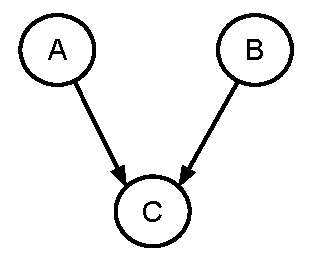
\includegraphics[width=0.15\textwidth]{Figures/nonequivalentClass}
		\end{center}
			\caption{V-structure: Two non-adjacent nodes converging to a common node become correlated. In the corresponding moral graph, they are bridged by an additional edge.}
					\label{fig:nonequivClass}
\end{figure}
\end{center}
\begin{algorithm}[H]
\caption{\textsc{DetriangulateMoralGraph}}
\label{algor:detriMoral}
\textbf{Input: $\mathcal{G} = (V, E)$, Correlation $\Sigma$, threshold $\sigma$} \\
\textbf{Output: A partially directed graph $\mathcal{G}^\prec$}\\\vspace{-4mm}
	\begin{algorithmic}[1]
		\FOR{each $e=(p, q)$ in $E$}
			\STATE $C \leftarrow \left\lbrace v_i \in V \,|\, v_i\text{ and } e\text{ form a triangle}\right\rbrace$ \\
				\FOR{colliders $\leftarrow \text{ each }k$-combination in $C$} 
					\STATE \algorithmiccomment{$k = 1,2,\ldots,|C|$}
					\STATE $N \leftarrow \left\lbrace v_i \in V \,|\, (v_i, p) \in E \text{ or } (v_i, q) \in E \right\rbrace$ \\
					\STATE $\hat{N} \leftarrow \left\lbrace \text{N}\setminus \text{colliders}\right\rbrace $\\
					\STATE $R \leftarrow$ $\Sigma_N^{-1}$
					\STATE $S \leftarrow$ $\Sigma_{\hat{N}}^{-1}$
					\STATE \algorithmiccomment{$\Sigma_S$ indicates the partial correlation matrix from $\Sigma$ with respect to set $S$}\\
					\IF{$S_{pq} < \sigma$}
						\IF{$R_{pq} > \sigma$}
							\STATE $E \leftarrow \left\lbrace E\setminus e\right\rbrace$
							\STATE orient $p$ and $q$ to all nodes in colliders
							\STATE break
						\ENDIF
					\ENDIF		
				\ENDFOR	
		\ENDFOR		
		\STATE return $\mathcal{G}^\prec \leftarrow \mathcal{G}$
	\end{algorithmic}
\end{algorithm}  

For each edge in a moral graph, it requires determining whether it is a bridged edge due to colliders or not. Suppose there is an edge $e_{ij}$ between node $i$ and $j$, denote the Markov blanket of both nodes as $M_{ij}$ and its potential colliders as $C_{ij}$ forming triangles with $e_{ij}$. Given $M_{ij}$, nodes $i$ and $j$ are $d$-separated from the other nodes. The partial inverse correlation matrix regarding the Markov blanket $M_{ij}$ encodes the conditional independences of $i$ and $j$. If now the colliders for nodes $i$ and $j$ are excluded from $M_{ij}$, then the inverse correlation matrix should be changed accordingly where additional information incurred by colliders will be now removed, in other words, $e_{ij}$ is a bridged edge. This can be done simply by comparing inverse correlation matrix regarding $\lbrace M_{ij} \setminus C_{ij}\rbrace$ with the one containing $C_{ij}$. Discovering the colliders will also orient nodes $i$ and $j$ towards its collider set $C_{ij}$. The pseudo-algorithm for the detriangulation is shown in Algorithm \ref{algor:detriMoral}.
Since a bridged edge could be due to multiple colliders, the algorithm iterates through $k$-combinations of colliders ($k$ starts from $1$ to the maximal number of potential colliders) until the real colliders are found, unless it is not a bridged edge. Note that the algorithm could be computationally intensive when the graph is fully connected.

\subsubsection{Constraint Propagation}
All the V-structures discovered from detriangulation will impose underlying constraints on the entire network. These constraints can be propagated through the network conforming to the following rules \cite{bkCausalityPearl}:
\vspace{-0.1in}
\begin{itemize}
\item $R_1$: Orient $a-b$ into $a\rightarrow b$ whenever there is an arrow $c\rightarrow a$ and $b$ and $c$ are not adjacent. (No new V-structure).
\vspace{-0.1in}
\item $R_2$: Orient $a-b$ into $a\rightarrow b$ whenever there is a path $a\rightarrow c \rightarrow b$. (Preserve the acyclicity)
\vspace{-0.1in}
\item $R_3$: Orient $a-b$ into $a\rightarrow b$ whenever there are two chains $a-c\rightarrow b$ and $a-d\rightarrow b$ such that $c$ and $d$ are not adjacent. (Three-fork structure)
\vspace{-0.1in}
\item $R_4$: Orient $a-b$ into $a\rightarrow b$ whenever there are two chains $a-c\rightarrow d$ and $c\rightarrow d \rightarrow b$ and $c$ and $b$ are not adjacent.
\vspace{-0.1in}
\end{itemize}  
% \begin{algorithm}[H]
\caption{\textsc{DetriangulateMoralGraph}}
\label{algor:detriMoral}
\textbf{Input: $\mathcal{G} = (V, E)$, Correlation $\Sigma$, threshold $\sigma$} \\
\textbf{Output: A partially directed graph $\mathcal{G}^\prec$}\\\vspace{-4mm}
	\begin{algorithmic}[1]
		\FOR{each $e=(p, q)$ in $E$}
			\STATE $C \leftarrow \left\lbrace v_i \in V \,|\, v_i\text{ and } e\text{ form a triangle}\right\rbrace$ \\
				\FOR{colliders $\leftarrow \text{ each }k$-combination in $C$} 
					\STATE \algorithmiccomment{$k = 1,2,\ldots,|C|$}
					\STATE $N \leftarrow \left\lbrace v_i \in V \,|\, (v_i, p) \in E \text{ or } (v_i, q) \in E \right\rbrace$ \\
					\STATE $\hat{N} \leftarrow \left\lbrace \text{N}\setminus \text{colliders}\right\rbrace $\\
					\STATE $R \leftarrow$ $\Sigma_N^{-1}$
					\STATE $S \leftarrow$ $\Sigma_{\hat{N}}^{-1}$
					\STATE \algorithmiccomment{$\Sigma_S$ indicates the partial correlation matrix from $\Sigma$ with respect to set $S$}\\
					\IF{$S_{pq} < \sigma$}
						\IF{$R_{pq} > \sigma$}
							\STATE $E \leftarrow \left\lbrace E\setminus e\right\rbrace$
							\STATE orient $p$ and $q$ to all nodes in colliders
							\STATE break
						\ENDIF
					\ENDIF		
				\ENDFOR	
		\ENDFOR		
		\STATE return $\mathcal{G}^\prec \leftarrow \mathcal{G}$
	\end{algorithmic}
\end{algorithm}  
% \begin{algorithm}[H]
\caption{\textsc{ConstraintPropagation}}
\label{algor:consProp}
\textbf{Input: a partially directed graph $\mathcal{G}^\prec$}\\
\textbf{Output: a maximally oriented graph $\mathcal{G}^\prec$}\\\vspace{-4mm}
	\begin{algorithmic}[1]
		\WHILE{$\mathcal{G}^\prec$ is changed}
					\IF{Edge($X$, $Y$) is undirected and $\exists$ directed path from $X$ to $Y$}
						\STATE set $X\rightarrow Y$ \algorithmiccomment{preserve acyclicity}\\  
						\STATE break	
					\ENDIF					
				\IF{$\exists$ node $X$ where $Y\rightarrow X\leftrightarrow Z$} 					
					\STATE set $Y\rightarrow X\rightarrow Z$ \algorithmiccomment{no new collider}\\ 
					\STATE break					
				\ENDIF		
					
				\IF{$\exists$ an undirected edge $X\leftrightarrow Y$ and \hfill\\ $\exists \text{ nonadjacent } Z \text{ and }W$ that $X\leftrightarrow Z\rightarrow Y$ and $X\leftrightarrow W\rightarrow Y$} 					
					\STATE orient as $X\rightarrow Y$ \algorithmiccomment{three-fork structure}\\
					\STATE break  	
				\ENDIF
		\ENDWHILE	
	%	\RETURN $\mathcal{G}^\prec$
	\end{algorithmic}
\end{algorithm}
Moreover, $R_4$ is not required, if the starting orientation is limited to V-structures. After constraint propagation, a maximally directed acyclic graph is formed. It does not require all the edges being directed. All the rules conform to either preserving the acyclicity or avoiding new V-structures. The pseudo-algorithm for constraint propagation is illustrated in Algorithm \ref{algor:consProp}.
% \begin{algorithm}[H]
\caption{\textsc{DetriangulateMoralGraph}}
\label{algor:detriMoral}
\textbf{Input: $\mathcal{G} = (V, E)$, Correlation $\Sigma$, threshold $\sigma$} \\
\textbf{Output: A partially directed graph $\mathcal{G}^\prec$}\\\vspace{-4mm}
	\begin{algorithmic}[1]
		\FOR{each $e=(p, q)$ in $E$}
			\STATE $C \leftarrow \left\lbrace v_i \in V \,|\, v_i\text{ and } e\text{ form a triangle}\right\rbrace$ \\
				\FOR{colliders $\leftarrow \text{ each }k$-combination in $C$} 
					\STATE \algorithmiccomment{$k = 1,2,\ldots,|C|$}
					\STATE $N \leftarrow \left\lbrace v_i \in V \,|\, (v_i, p) \in E \text{ or } (v_i, q) \in E \right\rbrace$ \\
					\STATE $\hat{N} \leftarrow \left\lbrace \text{N}\setminus \text{colliders}\right\rbrace $\\
					\STATE $R \leftarrow$ $\Sigma_N^{-1}$
					\STATE $S \leftarrow$ $\Sigma_{\hat{N}}^{-1}$
					\STATE \algorithmiccomment{$\Sigma_S$ indicates the partial correlation matrix from $\Sigma$ with respect to set $S$}\\
					\IF{$S_{pq} < \sigma$}
						\IF{$R_{pq} > \sigma$}
							\STATE $E \leftarrow \left\lbrace E\setminus e\right\rbrace$
							\STATE orient $p$ and $q$ to all nodes in colliders
							\STATE break
						\ENDIF
					\ENDIF		
				\ENDFOR	
		\ENDFOR		
		\STATE return $\mathcal{G}^\prec \leftarrow \mathcal{G}$
	\end{algorithmic}
\end{algorithm}  
It is very important to be aware of the order of applying these rules. The acyclicity should be the first and foremost of all the rules to be satisfied. Each time when an unknown edge is oriented, it should be followed by checking the acyclicity, or a cyclic graph could be created unintentionally.
\begin{algorithm}[H]
\caption{\textsc{ConstraintPropagation}}
\label{algor:consProp}
\textbf{Input: a partially directed graph $\mathcal{G}^\prec$}\\
\textbf{Output: a maximally oriented graph $\mathcal{G}^\prec$}\\\vspace{-4mm}
	\begin{algorithmic}[1]
		\WHILE{$\mathcal{G}^\prec$ is changed}
					\IF{Edge($X$, $Y$) is undirected and $\exists$ directed path from $X$ to $Y$}
						\STATE set $X\rightarrow Y$ \algorithmiccomment{preserve acyclicity}\\  
						\STATE break	
					\ENDIF					
				\IF{$\exists$ node $X$ where $Y\rightarrow X\leftrightarrow Z$} 					
					\STATE set $Y\rightarrow X\rightarrow Z$ \algorithmiccomment{no new collider}\\ 
					\STATE break					
				\ENDIF		
					
				\IF{$\exists$ an undirected edge $X\leftrightarrow Y$ and \hfill\\ $\exists \text{ nonadjacent } Z \text{ and }W$ that $X\leftrightarrow Z\rightarrow Y$ and $X\leftrightarrow W\rightarrow Y$} 					
					\STATE orient as $X\rightarrow Y$ \algorithmiccomment{three-fork structure}\\
					\STATE break  	
				\ENDIF
		\ENDWHILE	
	%	\RETURN $\mathcal{G}^\prec$
	\end{algorithmic}
\end{algorithm}
\begin{algorithm}[H]
\caption{\textsc{PICM-CBN Learning}}
\label{algor:copbn}
\textbf{Input: Dataset $D$, threshold $\sigma$} \\
\textbf{Output: All equivalent \textsc{DAGs}}\\\vspace{-4mm}
	\begin{algorithmic}[1]
		\STATE construct fully connected graph $\mathcal{G}$\\
		\STATE $marginals \leftarrow$ estimate marginals for each variable\\
		\STATE $\Sigma \leftarrow$ parameter estimation of Gaussian Copula\\
		\STATE $\Sigma^{-1} \leftarrow$ inverse correlation matrix $\Sigma$\\
		\FOR{each entry $e=\Sigma^{-1}_{ij}$}
			\IF{$e < \sigma$}
				\STATE remove $edge\left(i, j\right)$ from $\mathcal{G}$\\
			\ENDIF	
		\ENDFOR
		\STATE set Moral graph $\hat{\mathcal{G}} \leftarrow \mathcal{G}$\\	
		\STATE $\mathcal{G}^\prec \leftarrow $ DetriangulateMoralGraph($\hat{\mathcal{G}}, \Sigma, \sigma$)\\
		\STATE $\mathcal{G}^\prec \leftarrow $ ConstraintPropagation($\mathcal{G}^\prec$)\\
		\STATE \textsc{DAGs} $\leftarrow$ get equivalent graphs of $\mathcal{G}^\prec$\\
		\STATE return \textsc{DAGs}
	\end{algorithmic}
\end{algorithm} 

\subsubsection{Maximal DAG to Equivalent Networks}
The maximal DAG could possibly contain several equivalent graphs encoding the same joint probability distribution. Traditional structure learning methods will also end up with an equivalence class of networks. As a final step, it is worth converting the partial DAG (PDAG) to its equivalent completely oriented DAGs (CDAGs). This can be done using dynamic programming. Each undecided edge will be assigned an orientation manually, in the meantime, the constraints should always be updated and propagated. Thus it largely reduces the size of resulting networks and therefore is of great practical use. 
Finally, we present the PICM-CBN algorithm combining the Copula based parameter learning in Algorithm \ref{algor:copbn}. We adopted the Gaussian Copula. Note that, in Gaussian Copula, the estimated parameter $\Sigma$ can work as the input for the structure learning based on partial inverse correlation matrix. Thus we gain a significant improvement in running time. Even though there is a large number of missing observations, the learned parameters still suffice for the structure learning by applying a robust non-parametric density estimation on univariate marginals \cite{ElidanInferenceLess}.

\section{Experiments and Results}
\label{sec:expr}
This section presents the evaluation of the proposed algorithm on first, synthetic and
second, a real world data set.
The experiments on the synthetic data sets address the scalability and
parameter dependencies of the algorithm, while the second part on the real world data set compares the resulting network 
with prior knowledge in this domain and thus shows its applicability.

% 
% We present our experiment results in two parts, one of which was validated on synthetic 
% networks which were created with Bayesian network toolbox (BNT) \cite{bnt} and the training 
% data was also sampled by the toolbox. The other part is concerned with real world dataset. 
% However, the ground truth for real world dataset usually is hard to be captured. What we have 
% done is to construct a network which we can compare with our prior knowledge in this domain.

\subsection{Synthetic Networks}
The synthetic data sets comprise five
% We constructed five 
synthetic networks with node size $5, 7, 10, 20, 50$ which were created and
sampled with the Bayesian network toolbox (BNT) \cite{bnt}. This was 
repeated 10 times to examine data variability effects.
The size of the data sets (number of instances) ranges from  100 to 5000.
%
None of these 
networks represents a model of any real-world domain, 
 they are just created to represent causal relationships among variables. 
%
\begin{figure}[H]
\centering
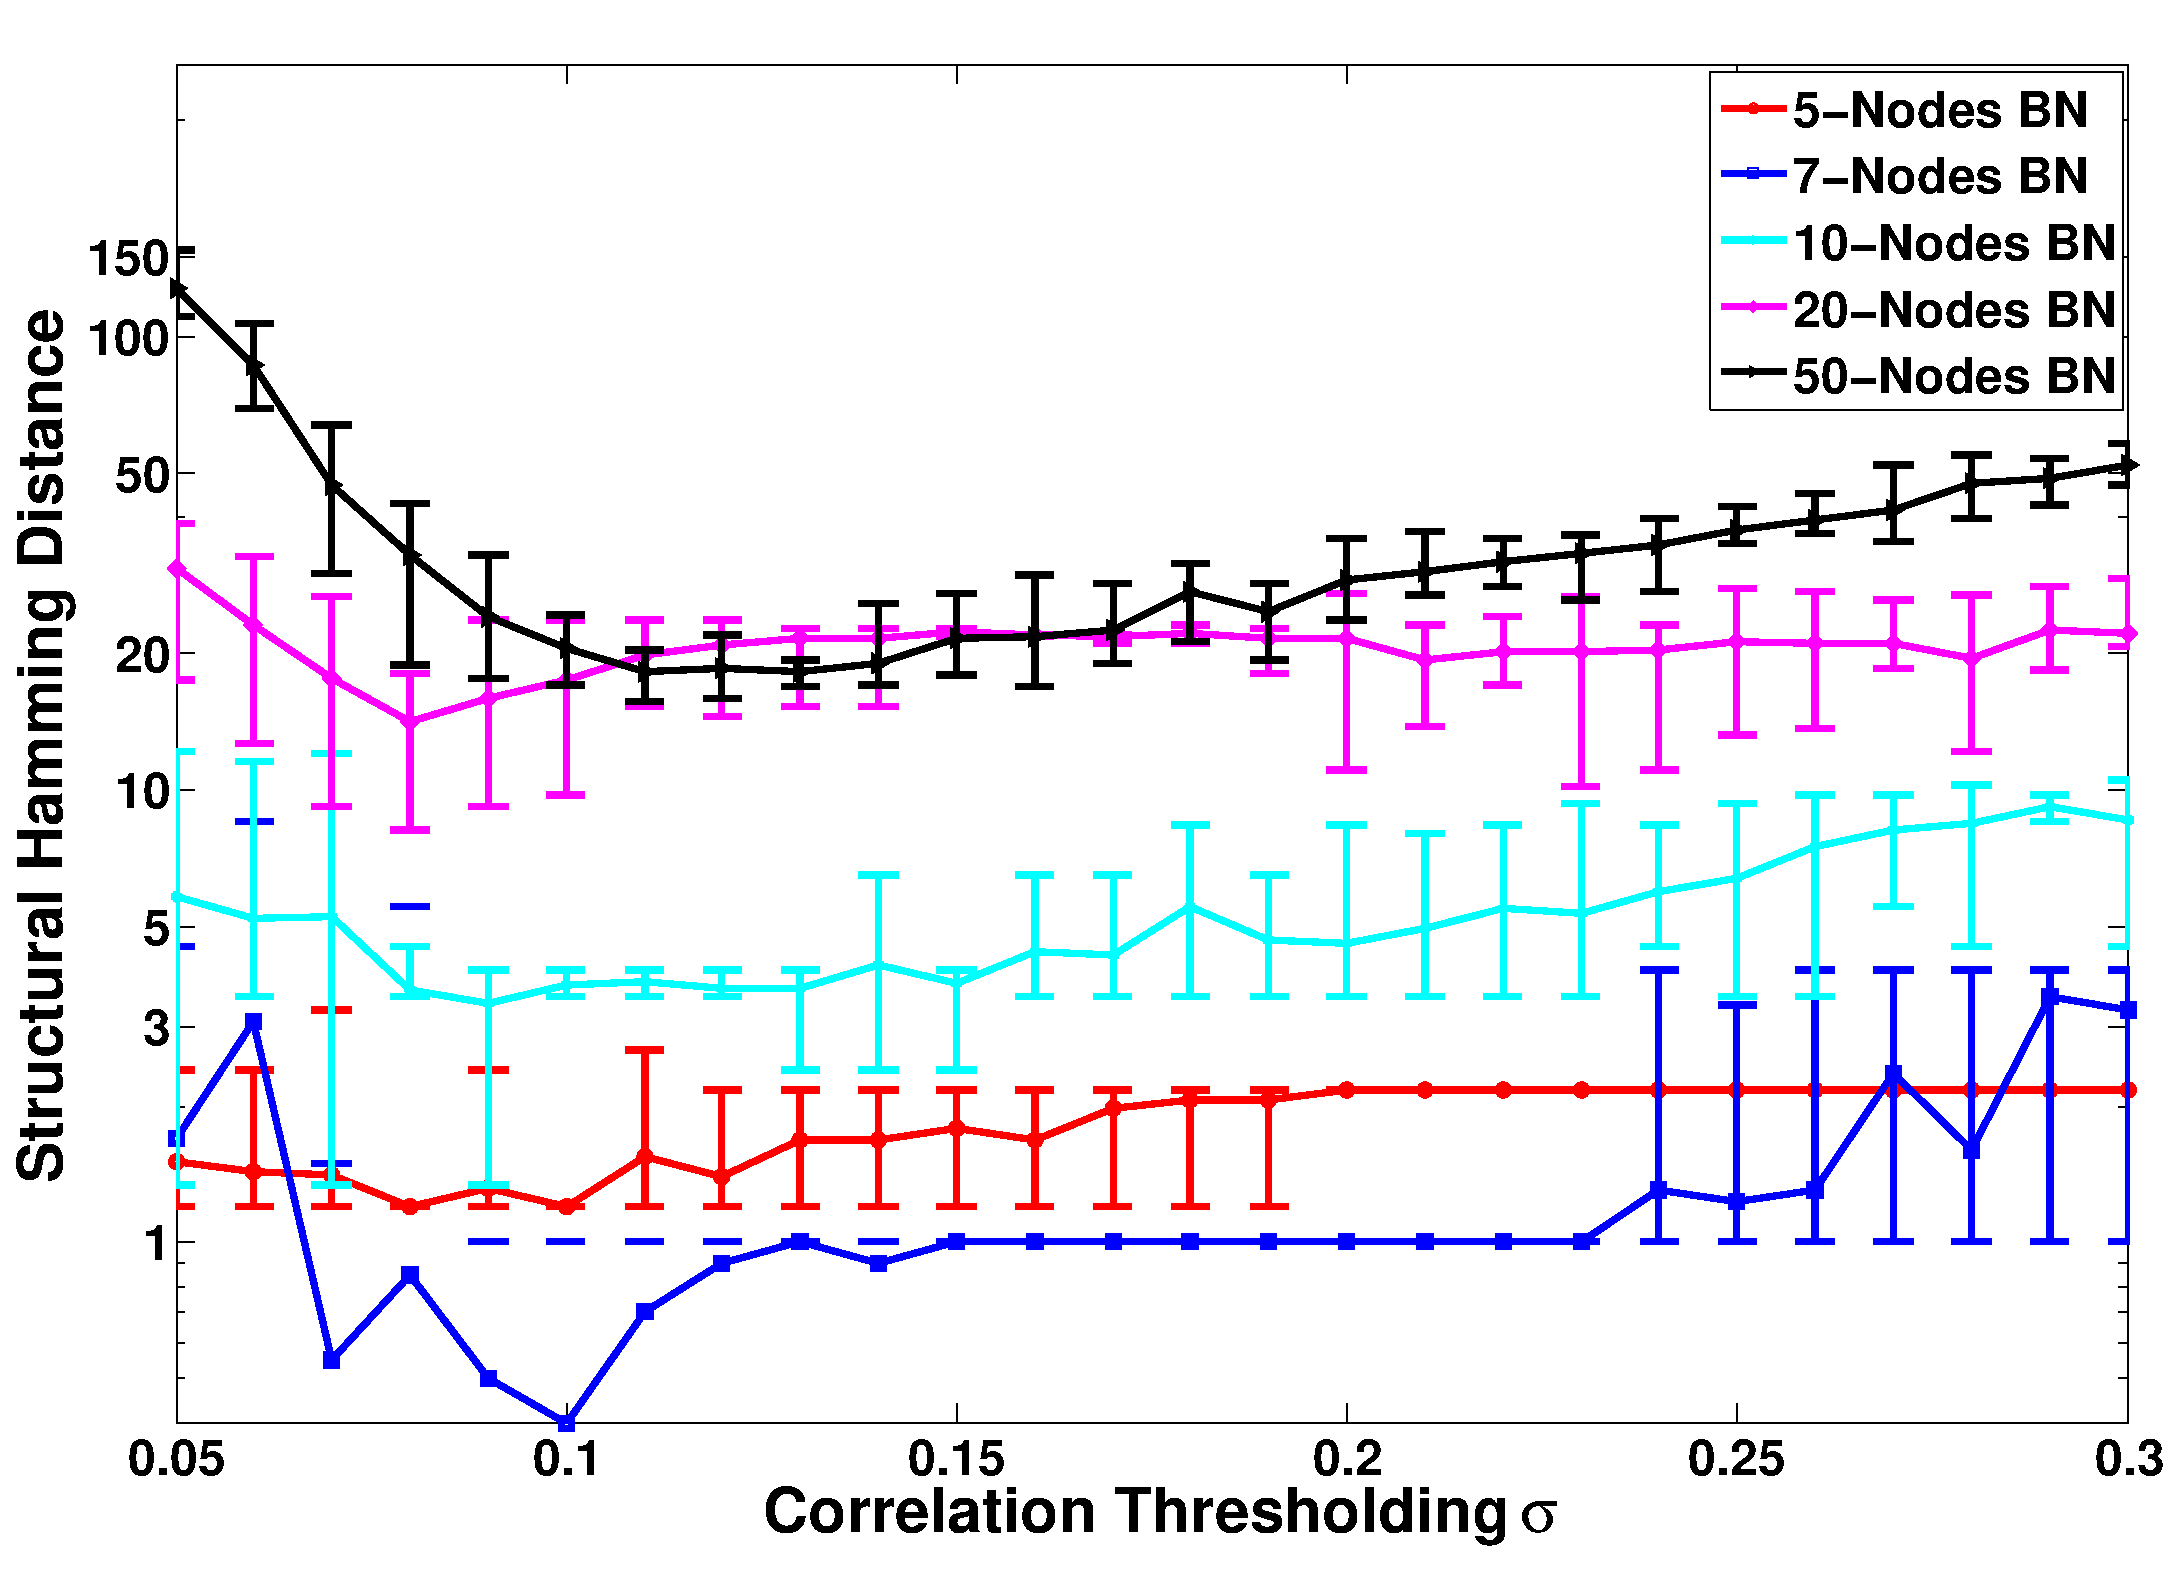
\includegraphics[width=0.4\textwidth]{Figures/plotsall/shd-alpha-errb}
\caption{SHD against $\sigma$ on five synthetic networks (node size 5, 7, 10, 20, 50, respectively) with training sample size  $ = 1000$ using PICM-CBN.}
\label{fig:shdAlphaResult}
\end{figure} \vspace{-0.2in}
In order to compare the learned structures with the original networks, we use the Structural  Hammming Distance (SHD) \cite{AcidCampos}, which calculates the minimal number of operations converting one network into another. 
One important parameter of the \textit{PICM-CBN} algorithm is the correlation zero-approximation threshold $\sigma$ (cf. Alg. \ref{algor:copbn})
that controls the number of edges in the graph. However, it is not obvious how to fix that threshold appropriately.
Therefore, the first evaluation examines the resulting networks by varying $\sigma$.
Figure \ref{fig:shdAlphaResult} shows that SHD approaches a 
minimum when $\sigma$ is around $0.1$, in the meantime, it achieves a stabler performance with less variance on SHD. For further experiments, $\sigma$ will be
fixed to the value of $0.1$, which is assumed to be reasonable.
\begin{figure}[H]
\centering
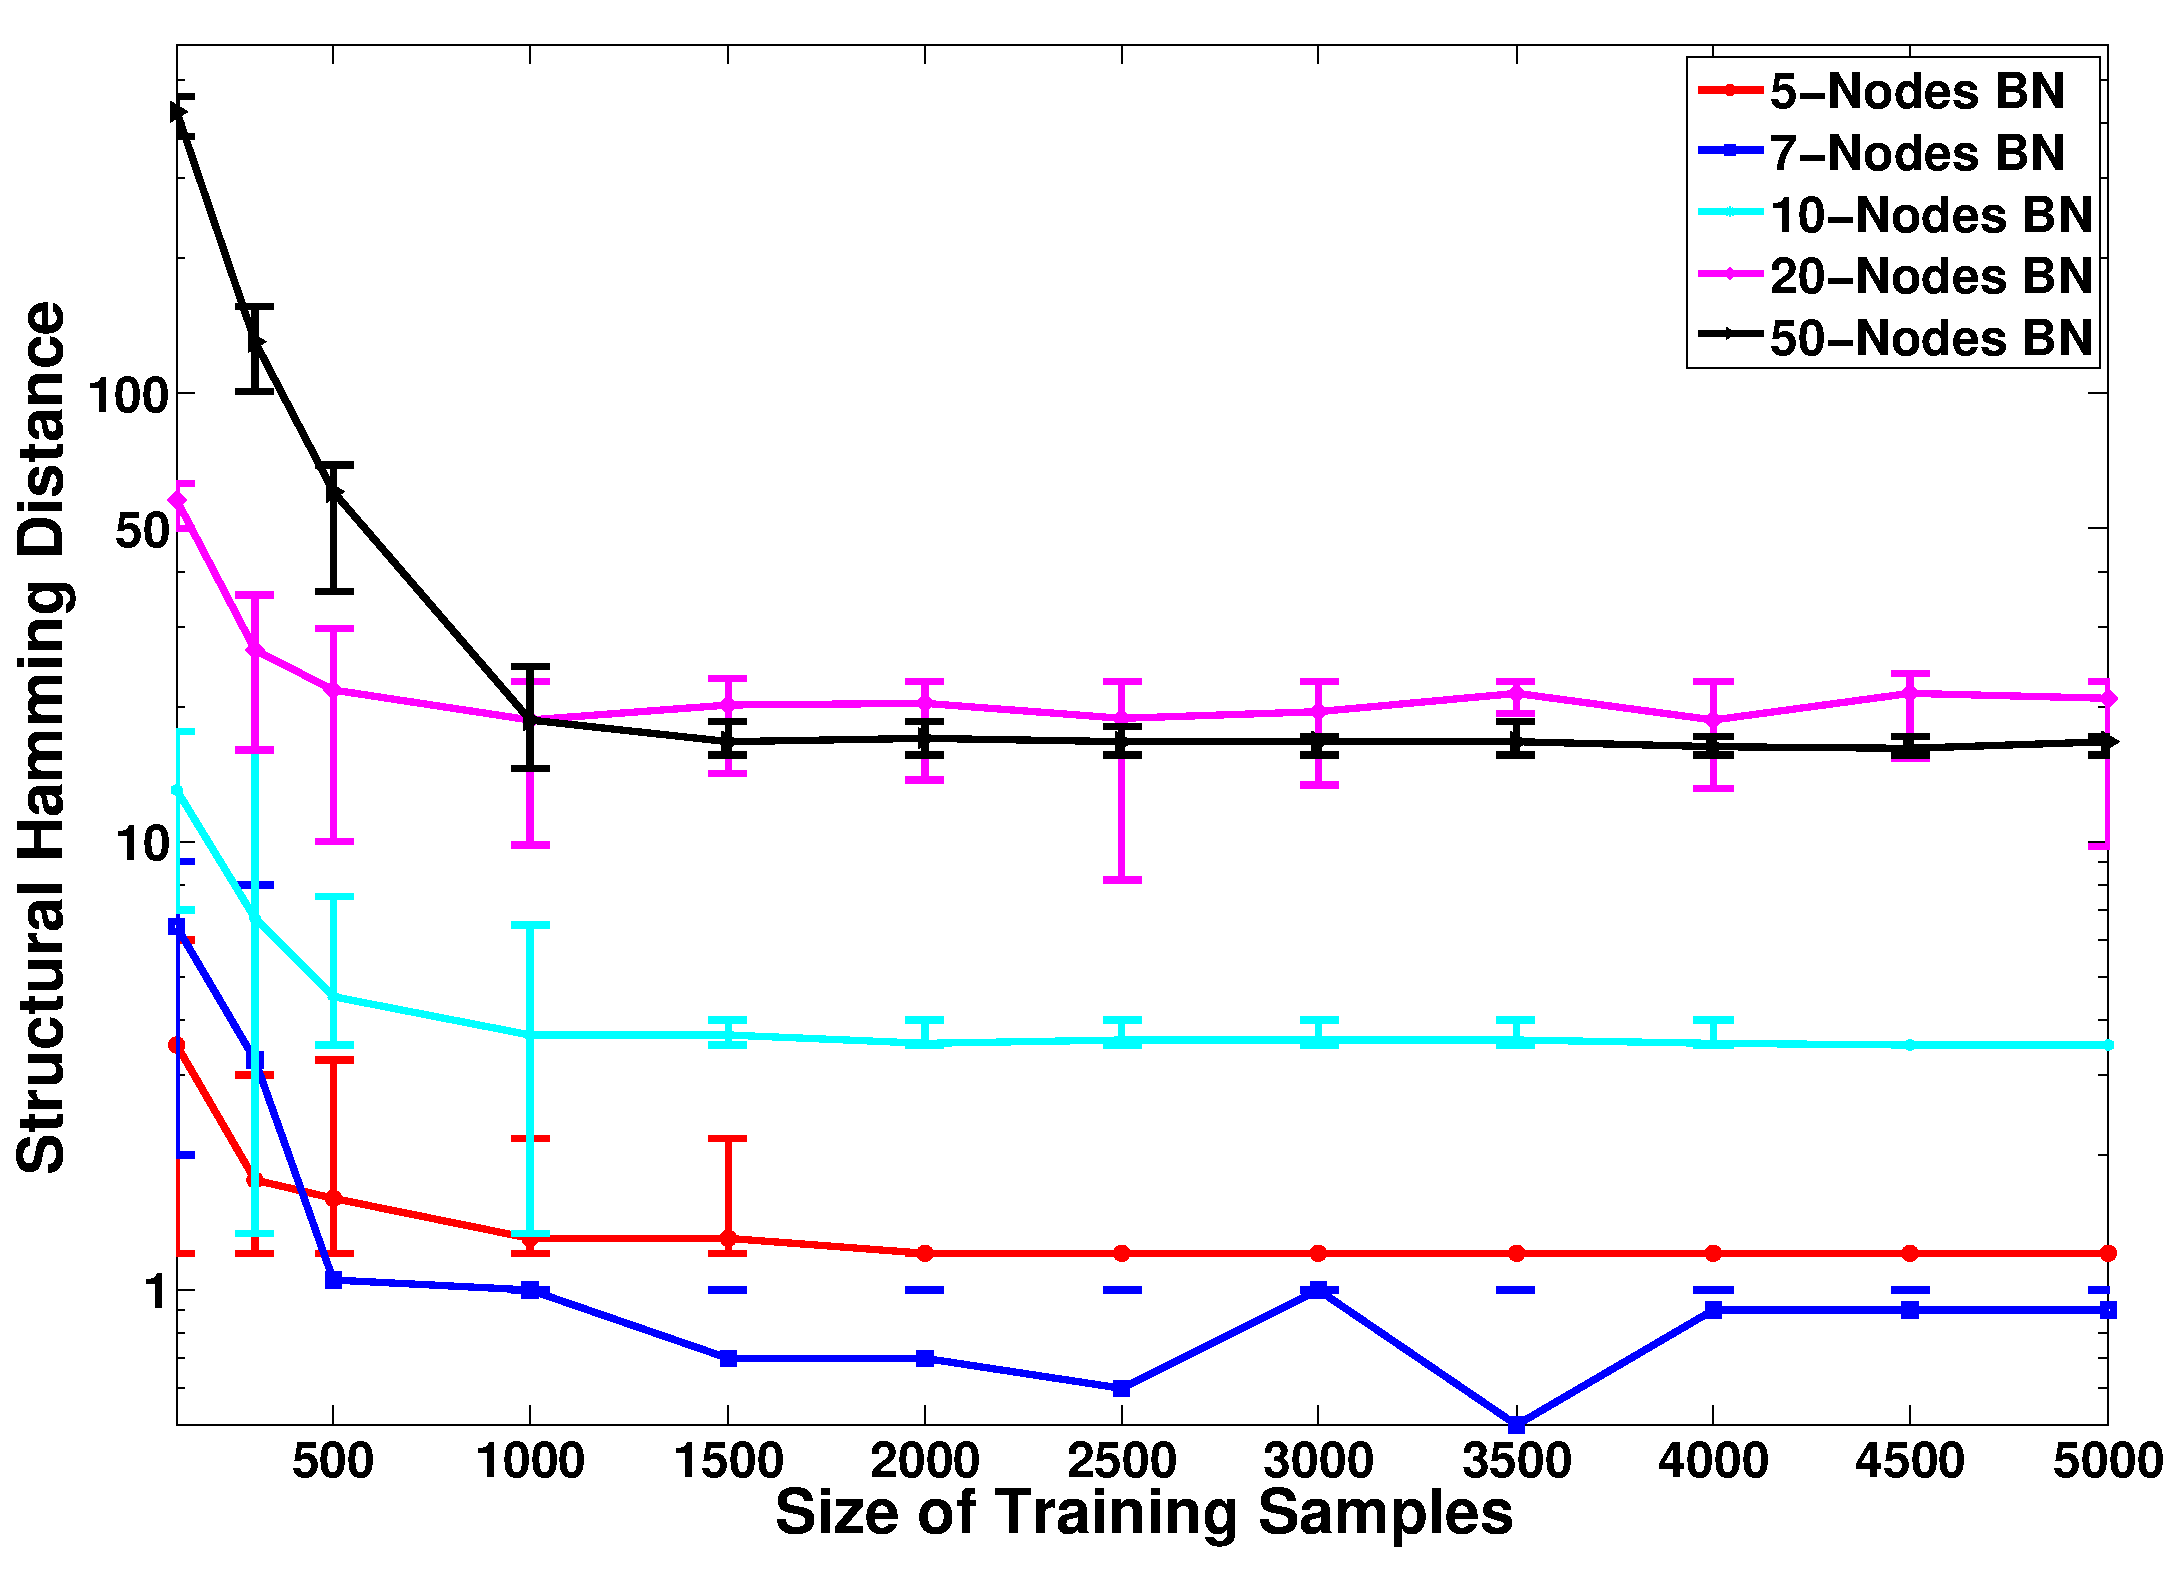
\includegraphics[width=0.4\textwidth]{Figures/plotsall/shd-samplesize-errb}
\caption{SHD against various training sample sizes on five synthetic networks (node size 5, 7, 10, 20, 50, respectively) using PICM-CBN ($\sigma = 0.1$). Sample size ranges from $100$ to $5000$.}
\label{fig:shdSampleResult}
\end{figure} 
\begin{figure}[H]
\centering
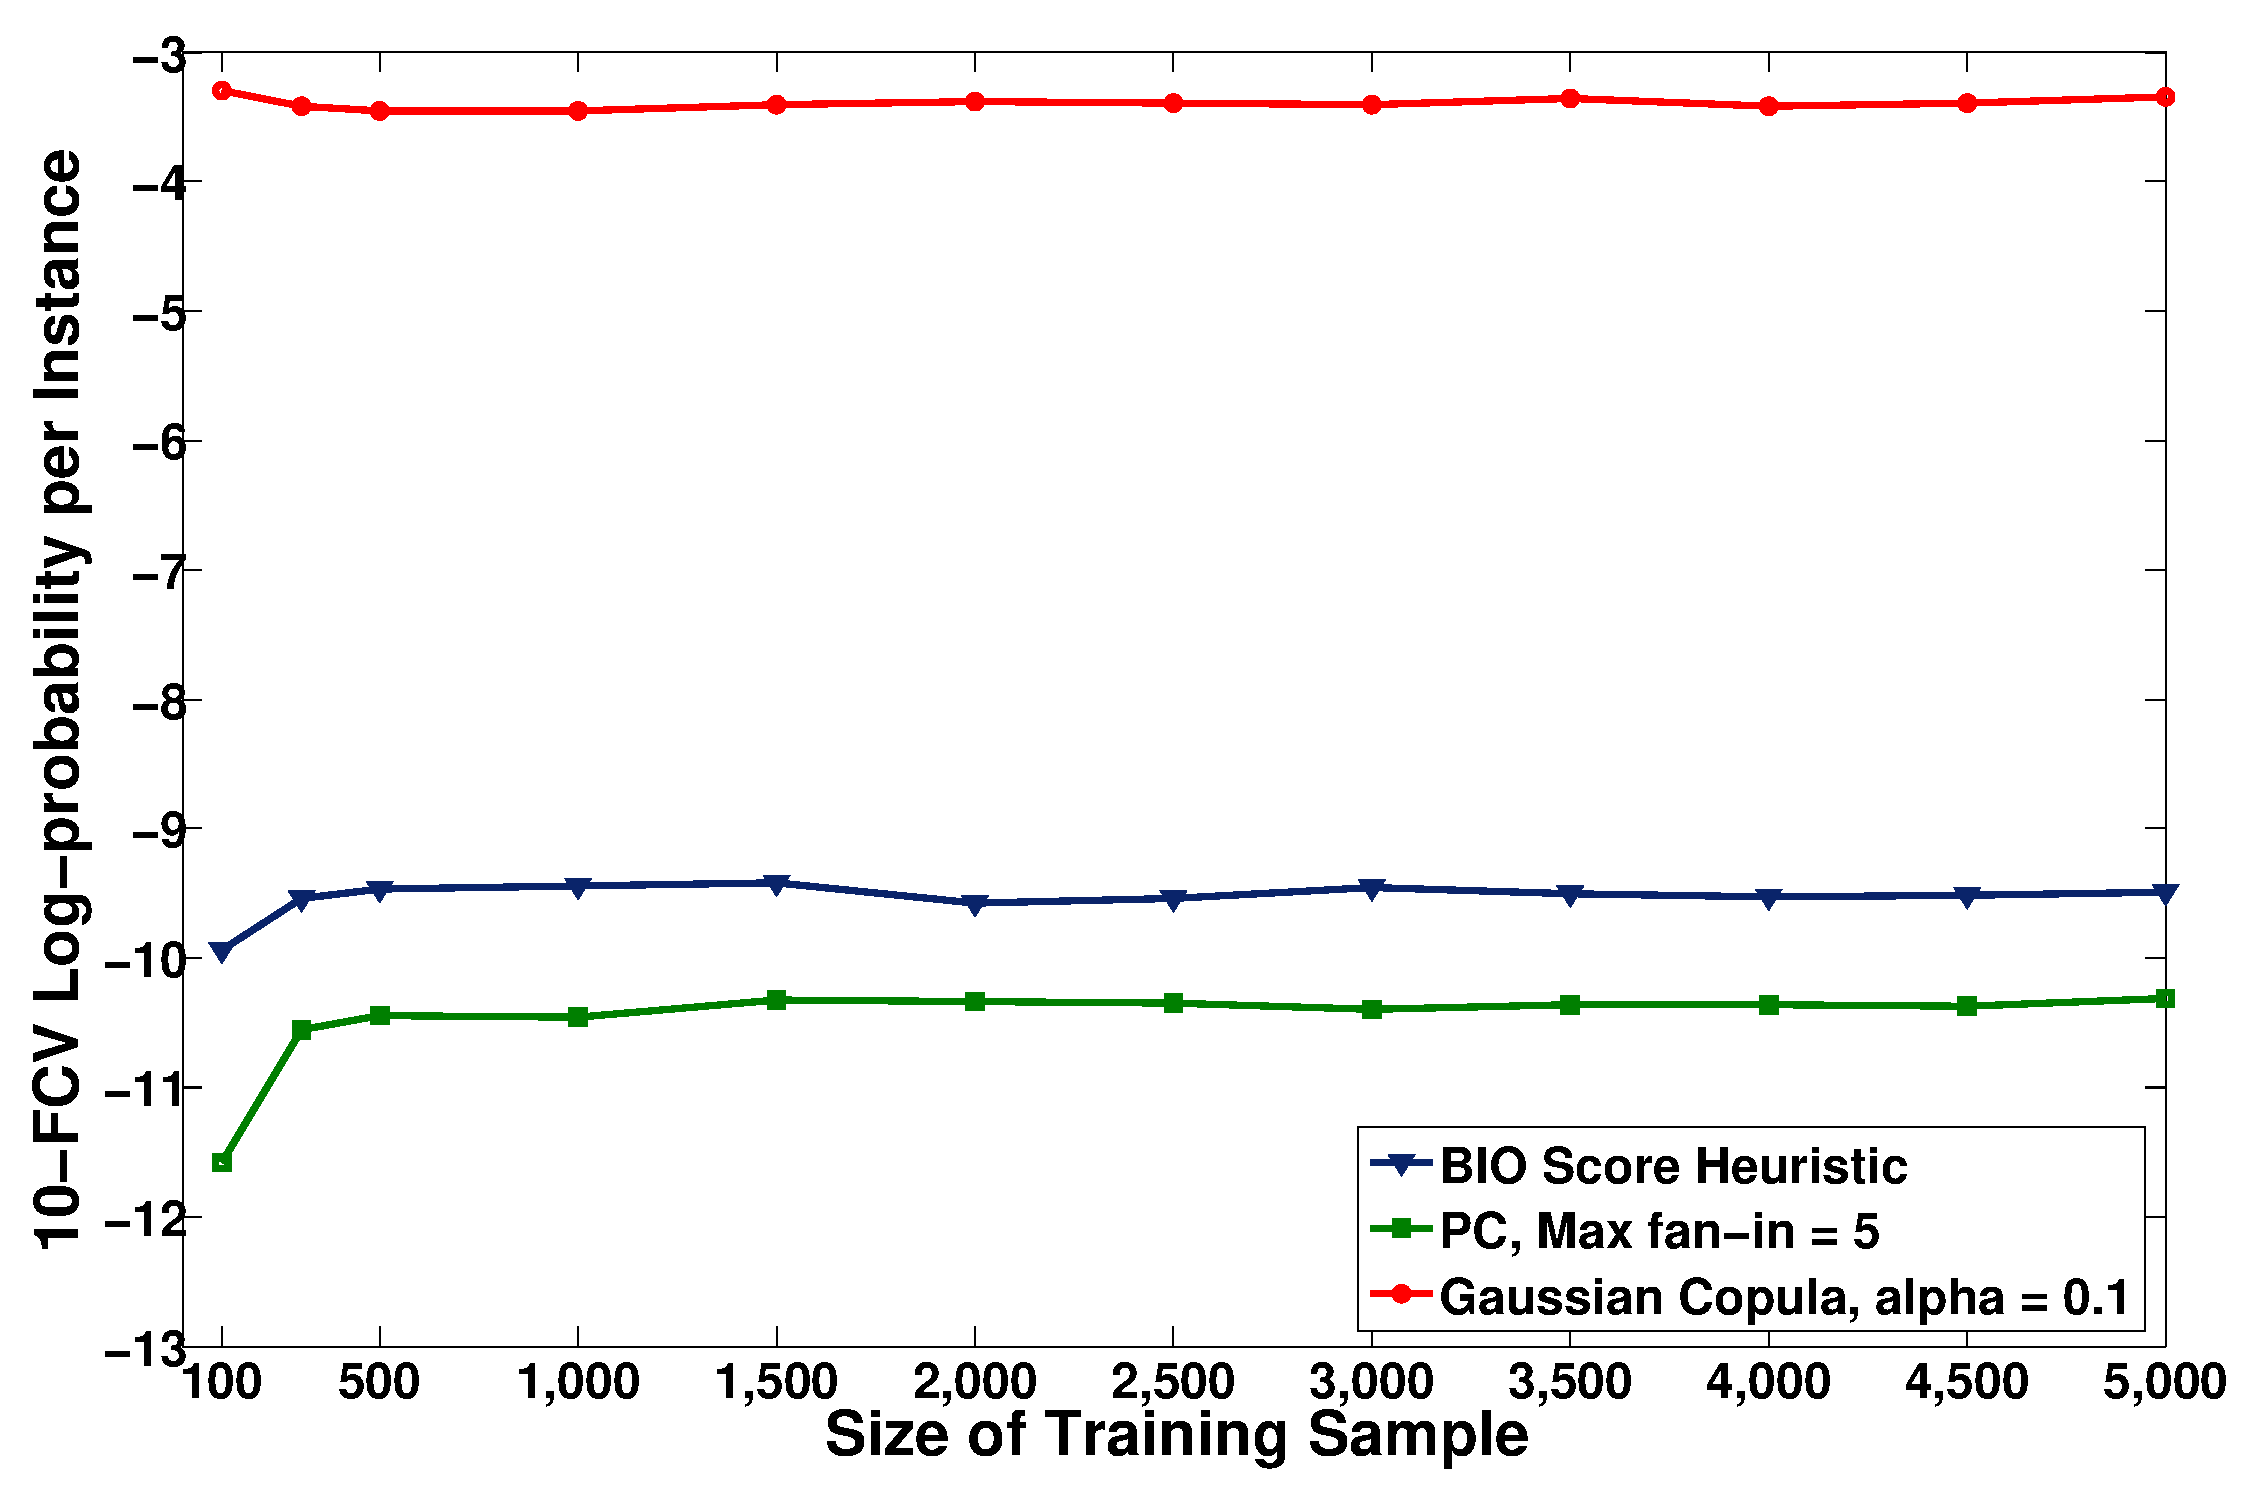
\includegraphics[width=0.4\textwidth]{Figures/plotsall/log-prob2}
\caption{
  Average log-probability per instance on testset against various training sample sizes (range from 100 to 5000) evaluated with 10FCV, on BIC scoring function 
  based heuristic BN Learning, PC Algorithm where Max-fan-in = 5 and thresholding $\alpha$ = 0.05, and also on 
  PICM-CBN BN learning, where correlation thresholding $\sigma = 0.1$.
}
\label{fig:logProb}
\end{figure} 
The next experiment addresses the algorithm's accuracy depending on the data set size.
Figure \ref{fig:shdSampleResult} shows that the SHD decreases for larger data sets and
reaches a promising value when the sample 
size exceeds 1000. Besides, for smaller sample size, the algorithm
 is not stable enough with high variances in SHD. 
Note that the SHD also correlates with the size of network, smaller networks are usually better identified than larger ones. In practice, a data set with a size above 500 should be considered as significant.

To evaluate the quality of the parameter learning, we ran experiments on data sets of various size using 10-fold cross-validation. We computed the average log-probability per instance over all test folds.
Let $lp$ denote the 
log-probability per instance in a test set $D_t$ of size $m$, then:
$lp = \frac{1}{|D_t|}\Sigma^m_{i=1}log(Pr(X_i))$, where $X_i$ is the $i$-th instance in $D_t$. PC algorithm and BIC score function based method were taken for comparison. Both of these two algorithms adopt MLE as parameter estimation strategy. Since BIC score heuristic method is computationally quite demanding for learning large networks, this experiment was only run on the 5-Nodes network. It is obvious from Figure \ref{fig:logProb} that Copula based parameter estimation outperforms the other two on any training sample size.

Additionally, Figure \ref{fig:costplots} shows Precision, Recall and the error rate
of SHD against various $\sigma$ on the five synthetic data sets.
 \begin{figure*}
 \centering{
   \subfigure[Precision]{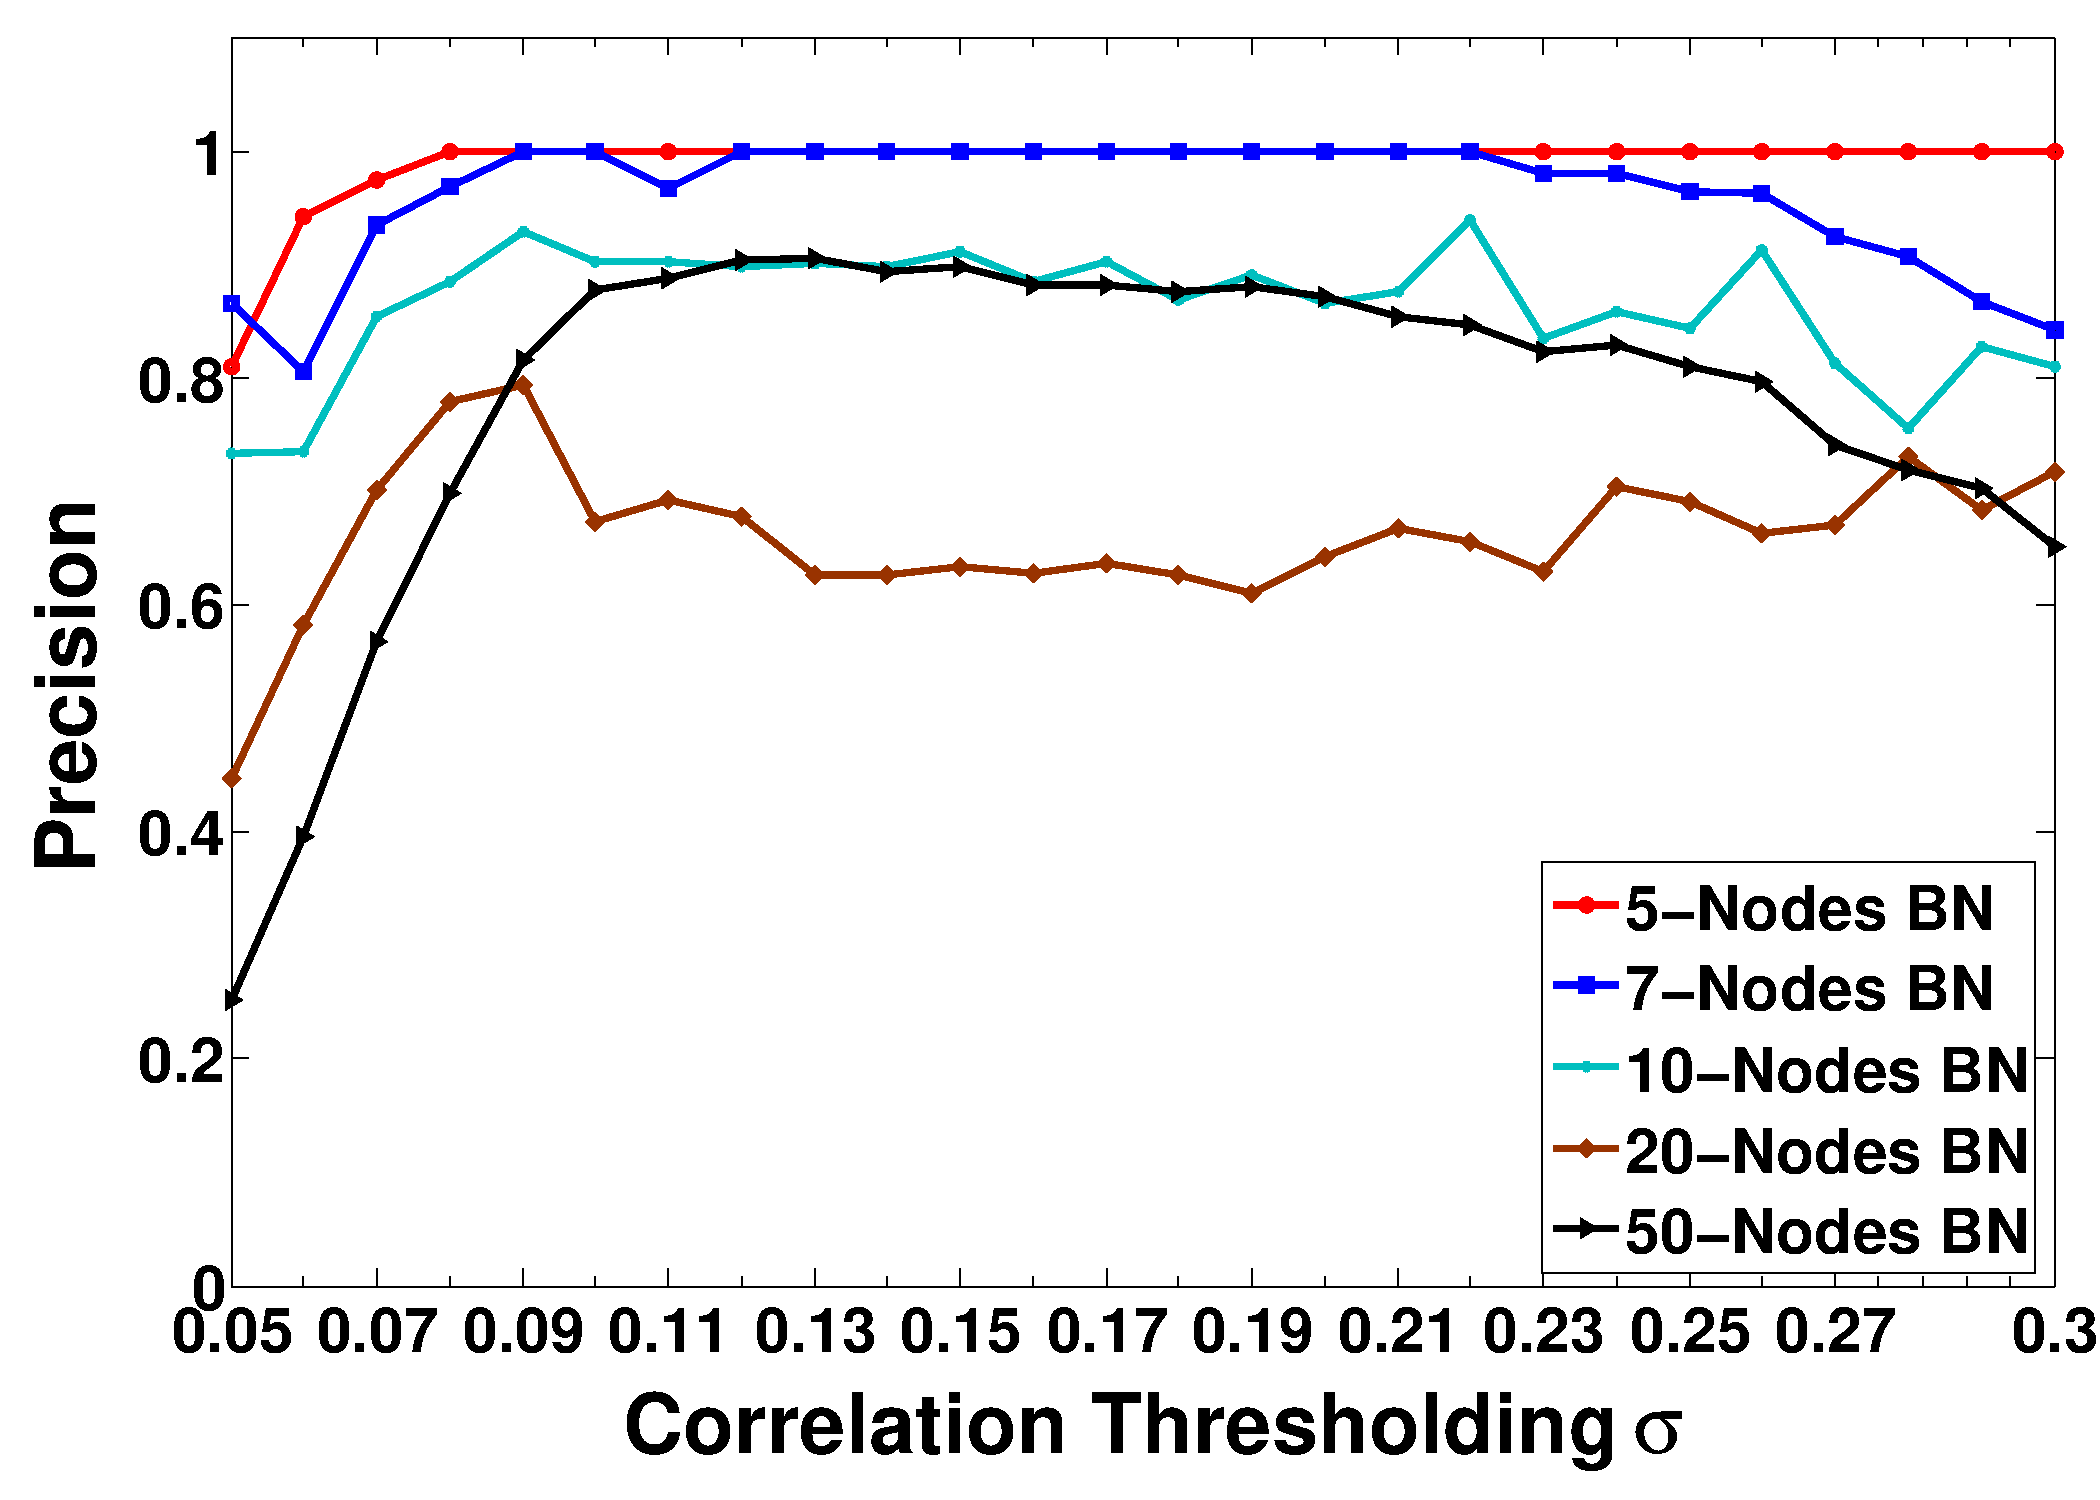
\includegraphics[width=0.326\textwidth]{Figures/plotsall/precision-copula}}
 % }
 % \centering{
   \subfigure[Recall]{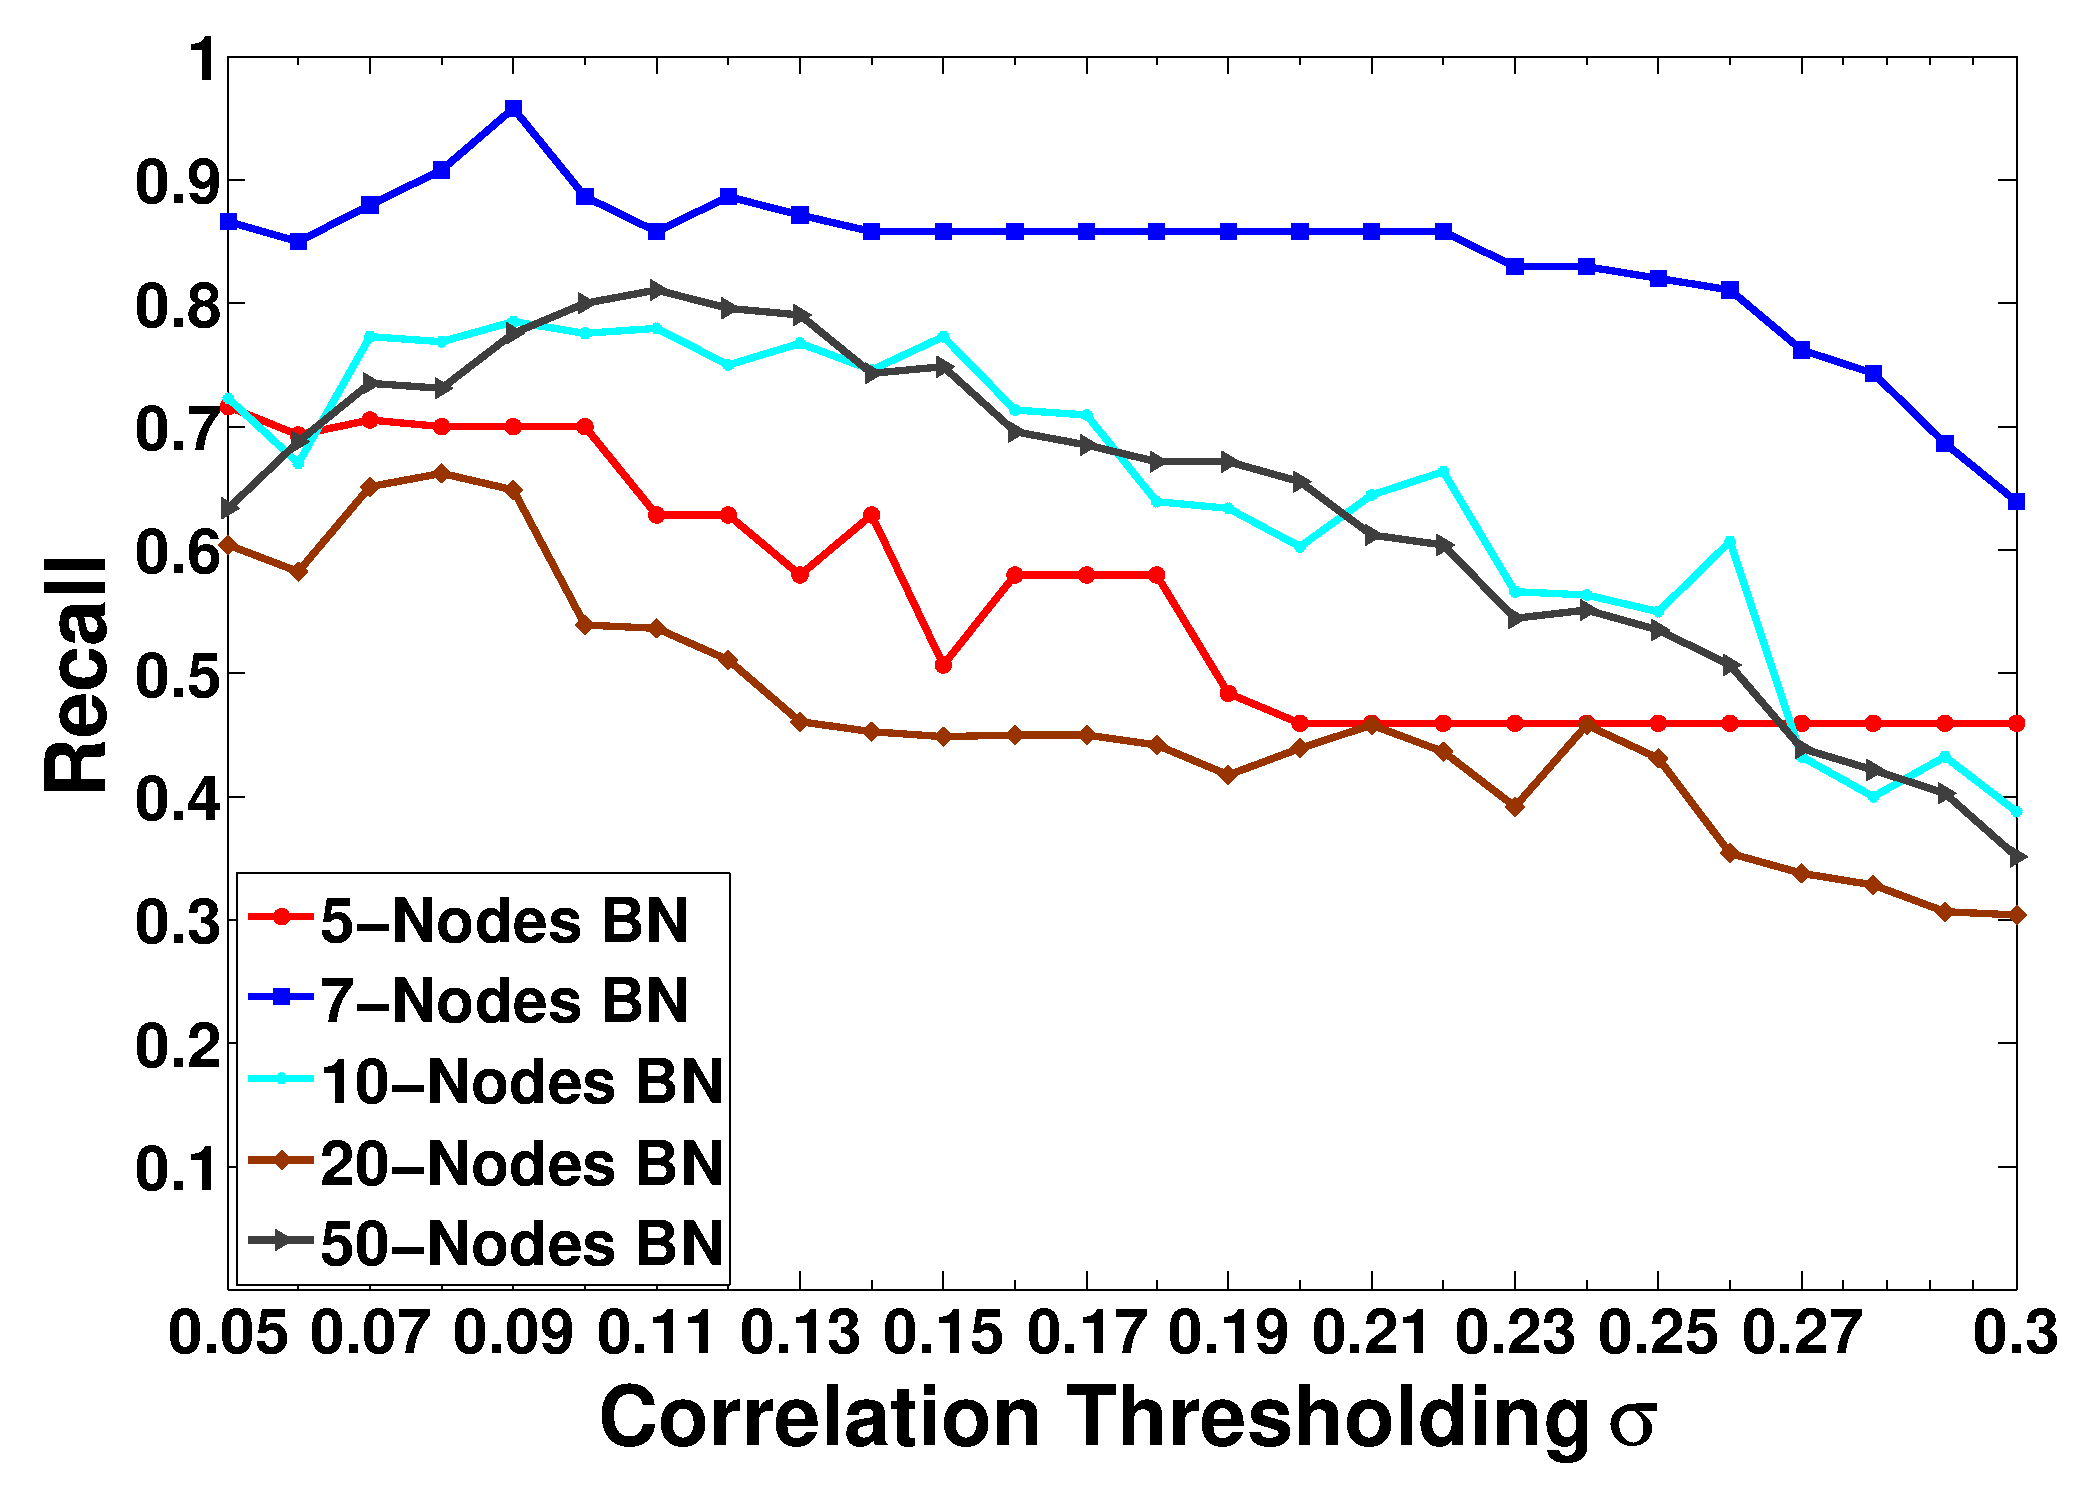
\includegraphics[width=0.33\textwidth]{Figures/plotsall/recall-copula}}
 % }
 % \centering{
   \subfigure[Error rate]{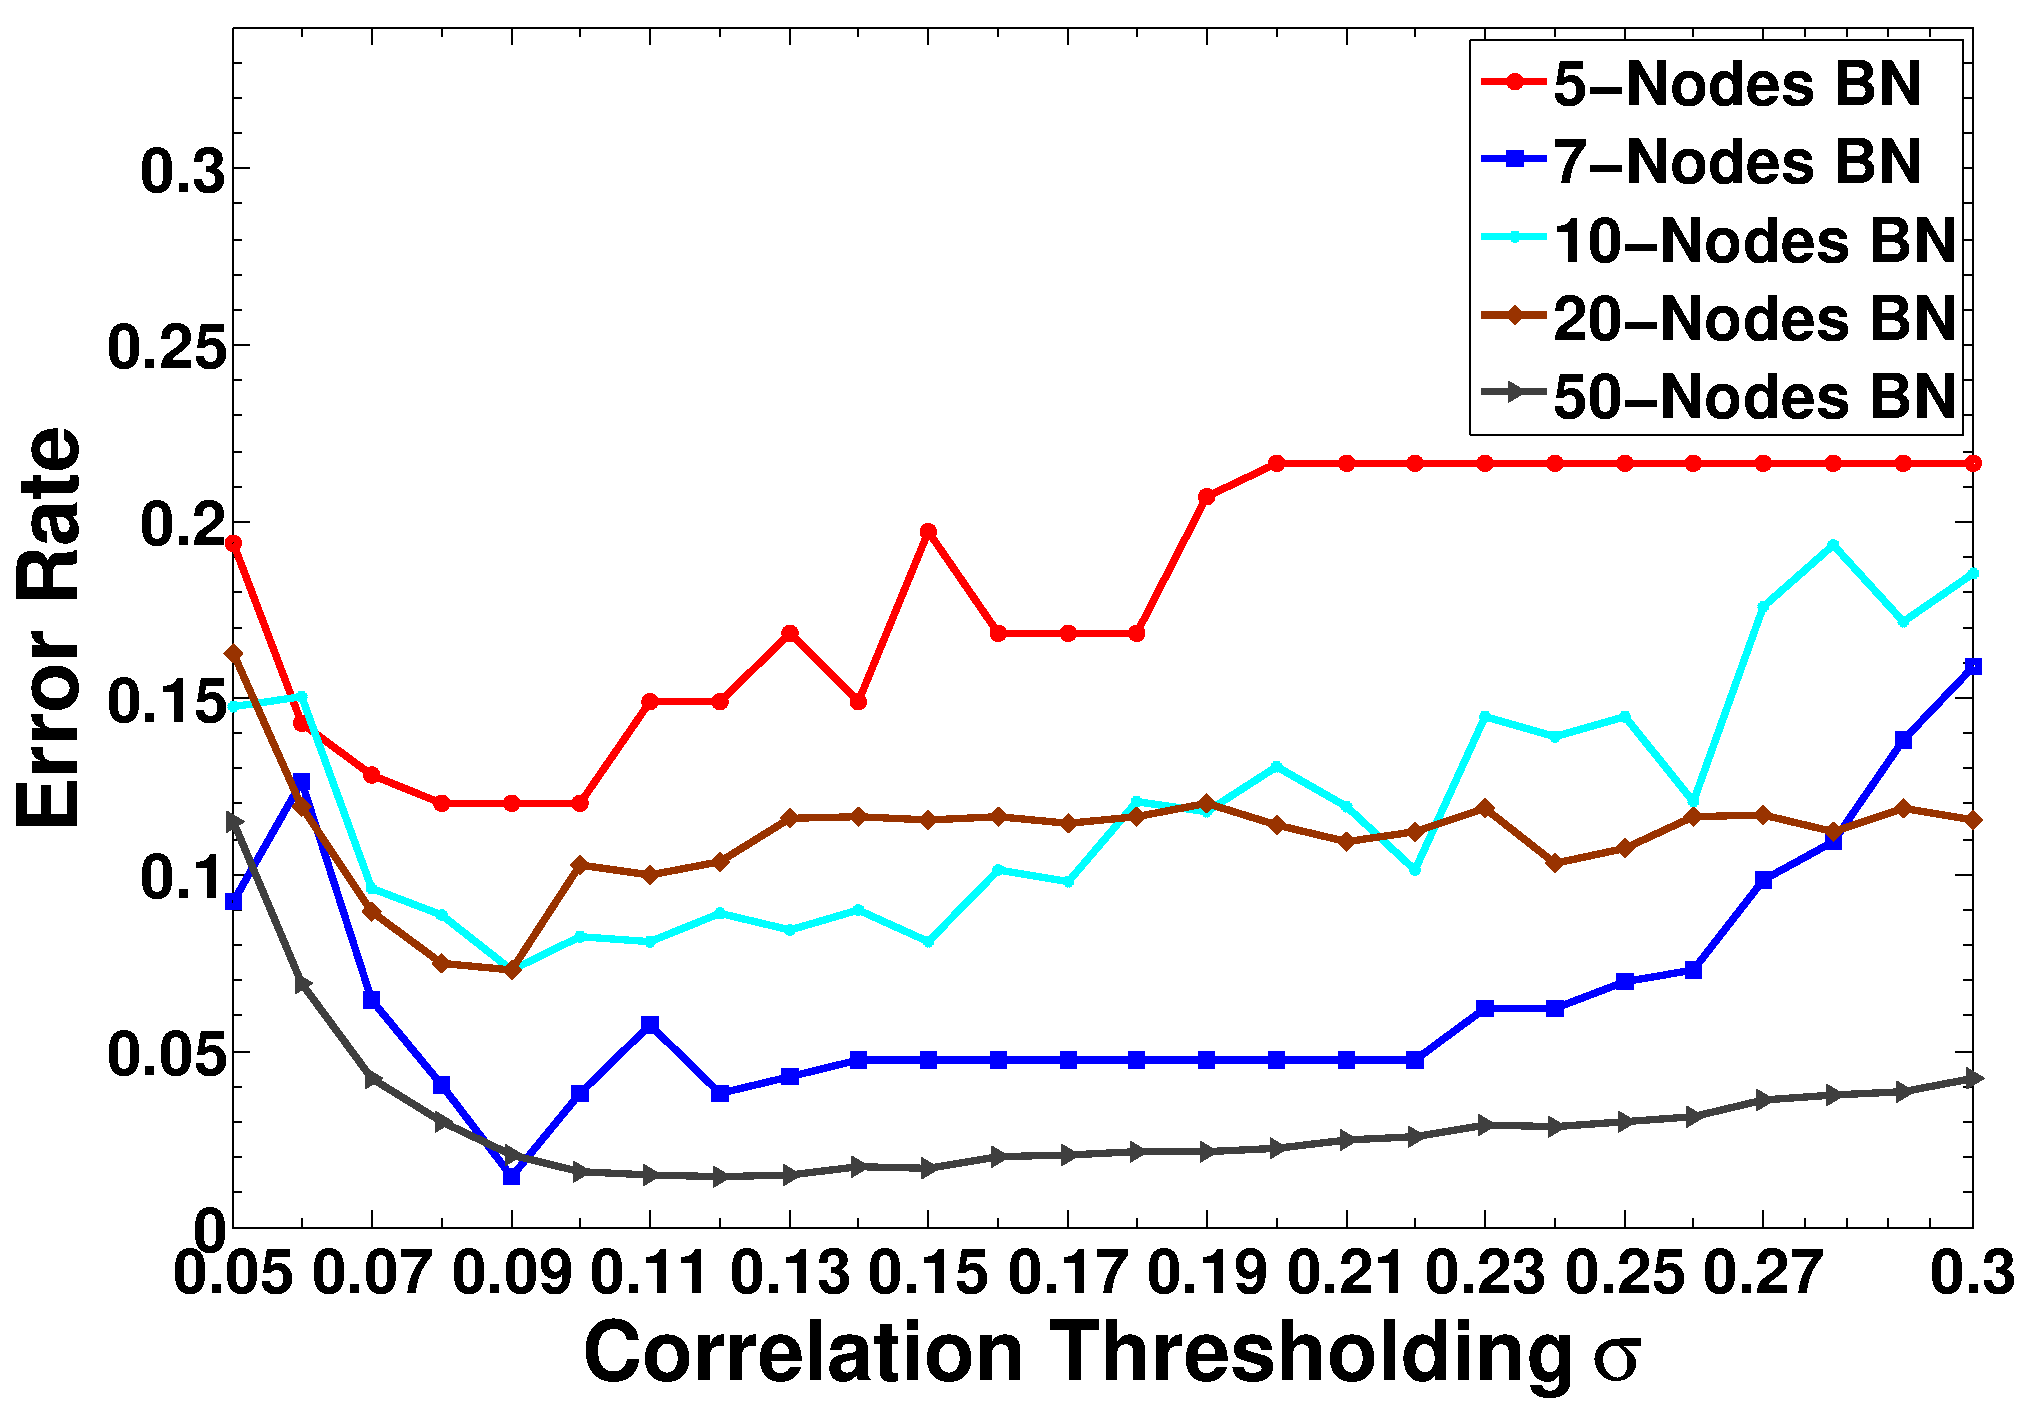
\includegraphics[width=0.33\textwidth]{Figures/plotsall/ErrorRate-copula}}
 }
 \caption[centerlast]{Precision (a), Recall (b) and error rate (c) against various $\sigma$ ranging from 0.05 to 0.3 on five synthetic networks (node size 5, 7, 10, 20, 50) with training sample size $= 1000$ using PICM-CBN.}
 \label{fig:costplots}
 \end{figure*} 
% In Figure \ref{fig:costplots}, e
Even the 50-Nodes network approaches a precision of 0.9 when 
$\sigma$ is around 0.1. This means that 90\% of the inferred edges appear indeed in the original network.
% are indeed in gold standard 
% network. 
The Recall values for all the learned networks except the 5-Nodes and 20-Nodes stay 
beyond 0.7 when the $\sigma$ is around 0.1. This indicates that over 70\% edges of 
original networks can be correctly inferred. The error rate represents the total accuracy of learned structures,
mostly it is beneath 0.1, which corresponds to 90\% accuracy.

The last experiment compares the \textit{PICM-CBN} algorithm with the PC algorithm on the 
synthetic networks of size 5, 7, and 10.
% We show 
% the notability of PICM-CBN both in structure learning and computational efficiency. 
Figure \ref{fig:runtime} gives the runtimes and the SHD.
 PICM-CBN performs slightly better on structure learning than the PC algorithm for these small sized networks,
 and remarkably better in terms of runtime. Moreover, PICM-CBN is also more stable than PC, especially
 when the data set size is above $1000$. %reaches a significant level ($>1000$). 

\subsection{Real World Data Set}
\label{sec:ExpRealWorld}
% Experiments conducted on synthetic BNs have shown the expected advantages of the PICM-CBN learning method 
% both on parameter estimation and structure learning. 
% 
The second experiment part was run on the Abalone 
data set \cite{abaloneBook} taken from UCI repository \cite{uciRepo}. The Abalone data set contains 
4177 samples and 9 attributes in total, of which there is one nominal attribute indicating the sex of abalone, which was removed for this experiment. The original task of this data set is to predict the age of an abalone, which is usually done by counting the number of rings of the abalone. Again, the PC algorithm was taken for comparison. 
Figure \ref{fig:abalonelp} shows the log-probability of the induced networks for both algorithms. 
\begin{figure}[H]
\centering
\subfigure[5-nodes: runtime]{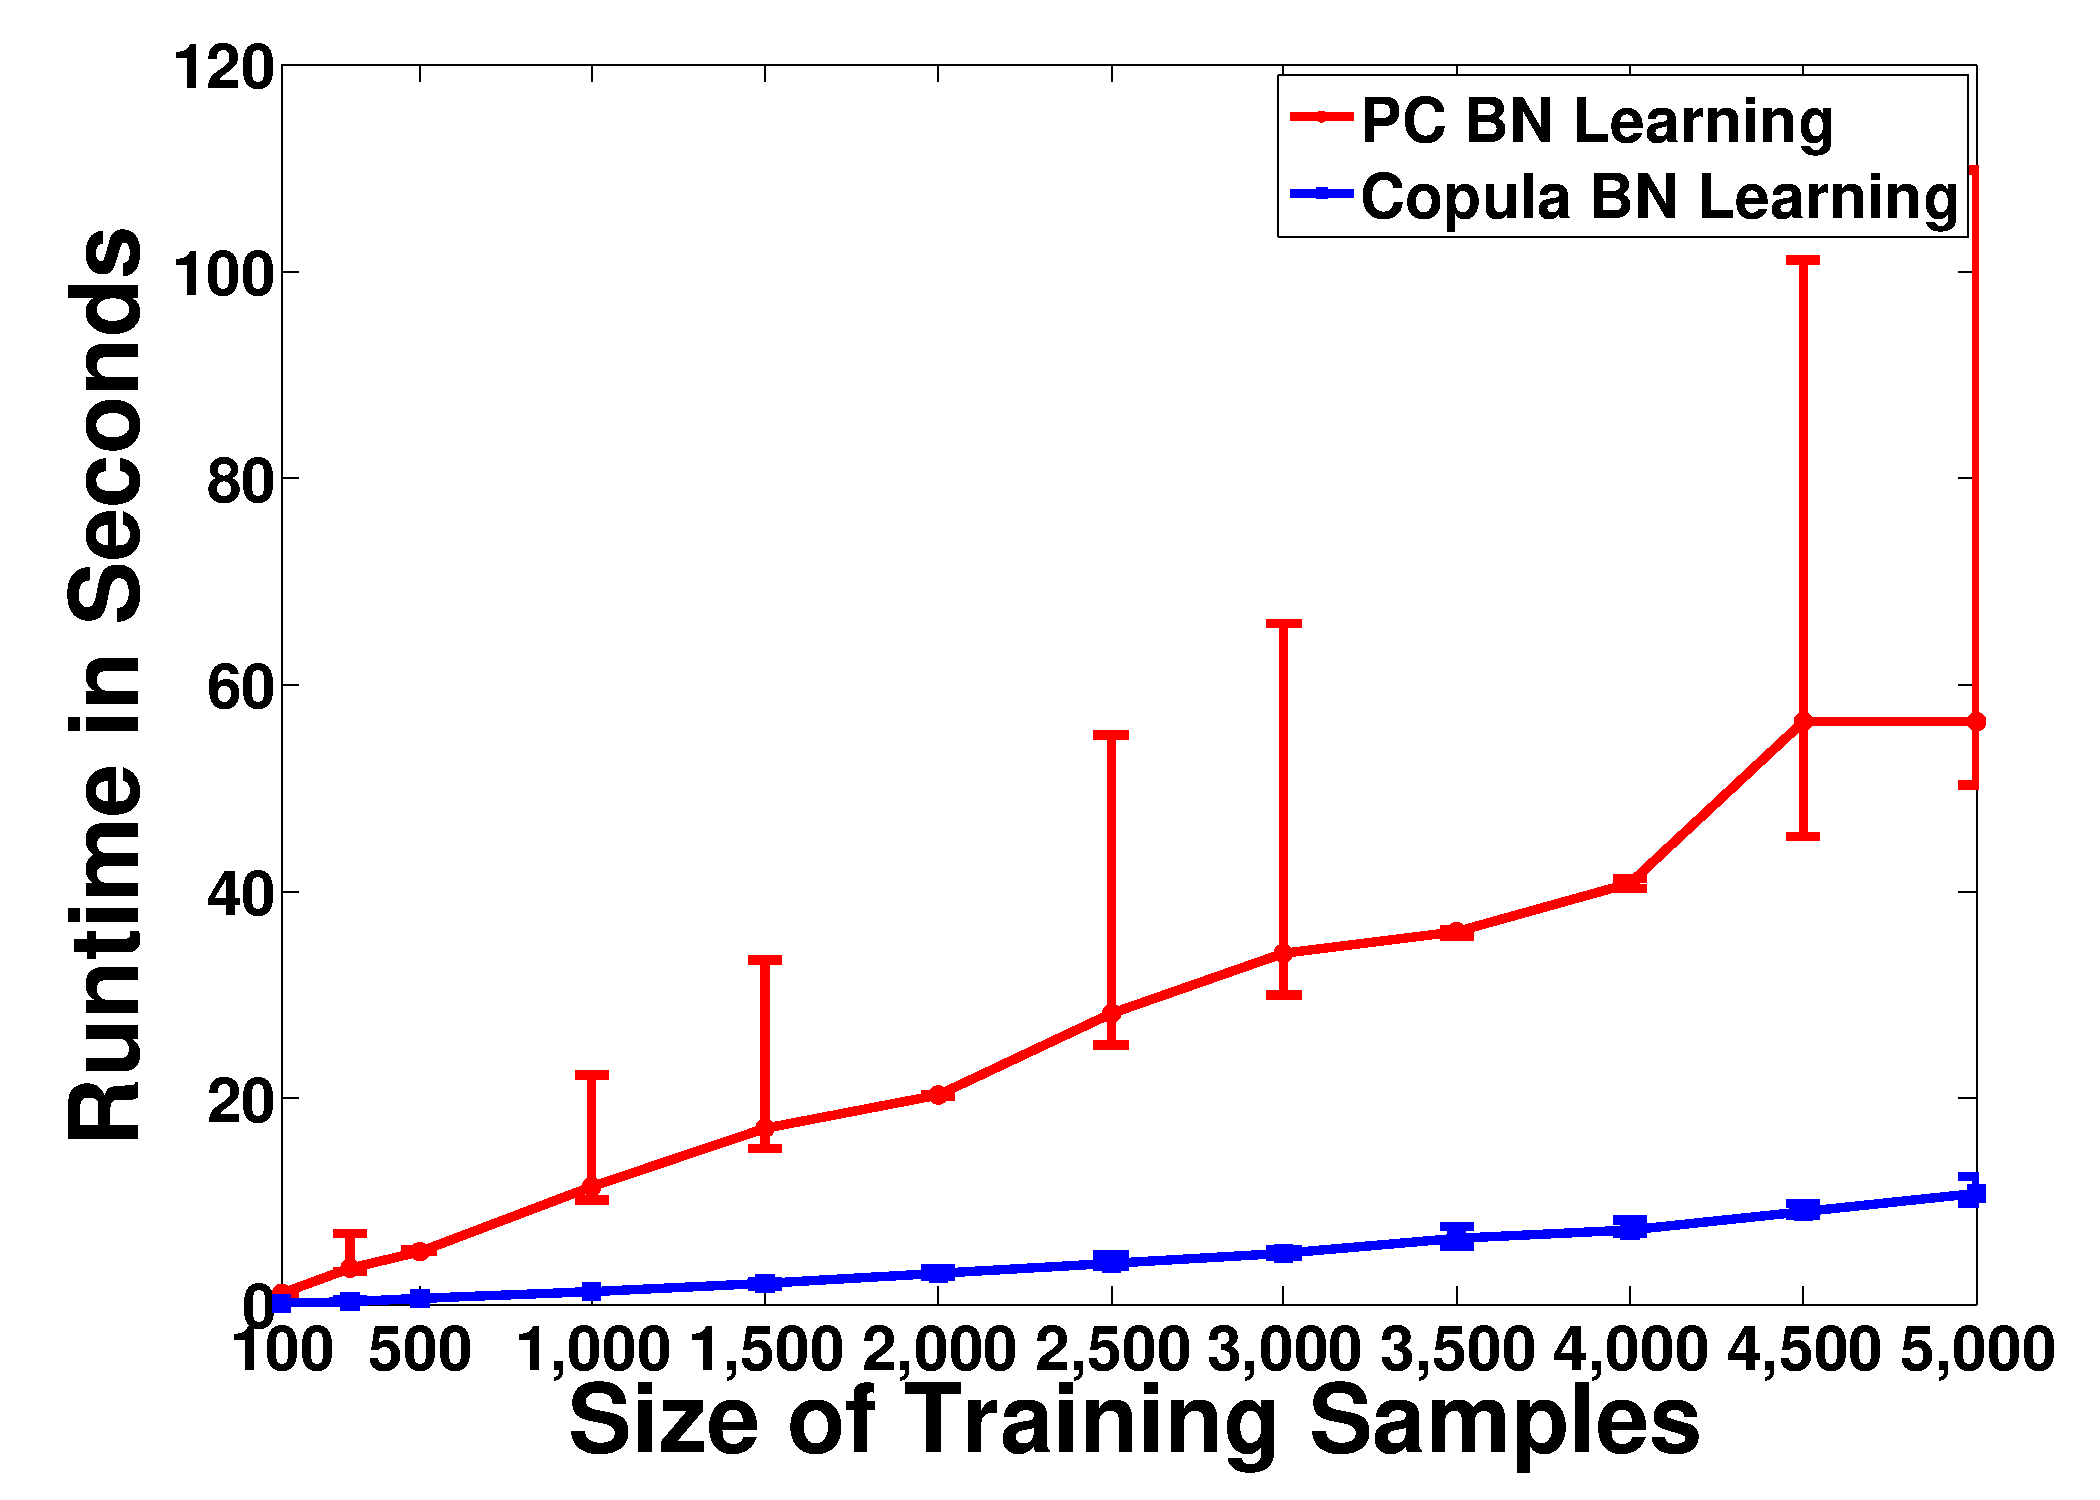
\includegraphics[width=0.24\textwidth]{Figures/plotsall/rtime-5err-f100}}\hfill
\subfigure[5-nodes: SHD error]{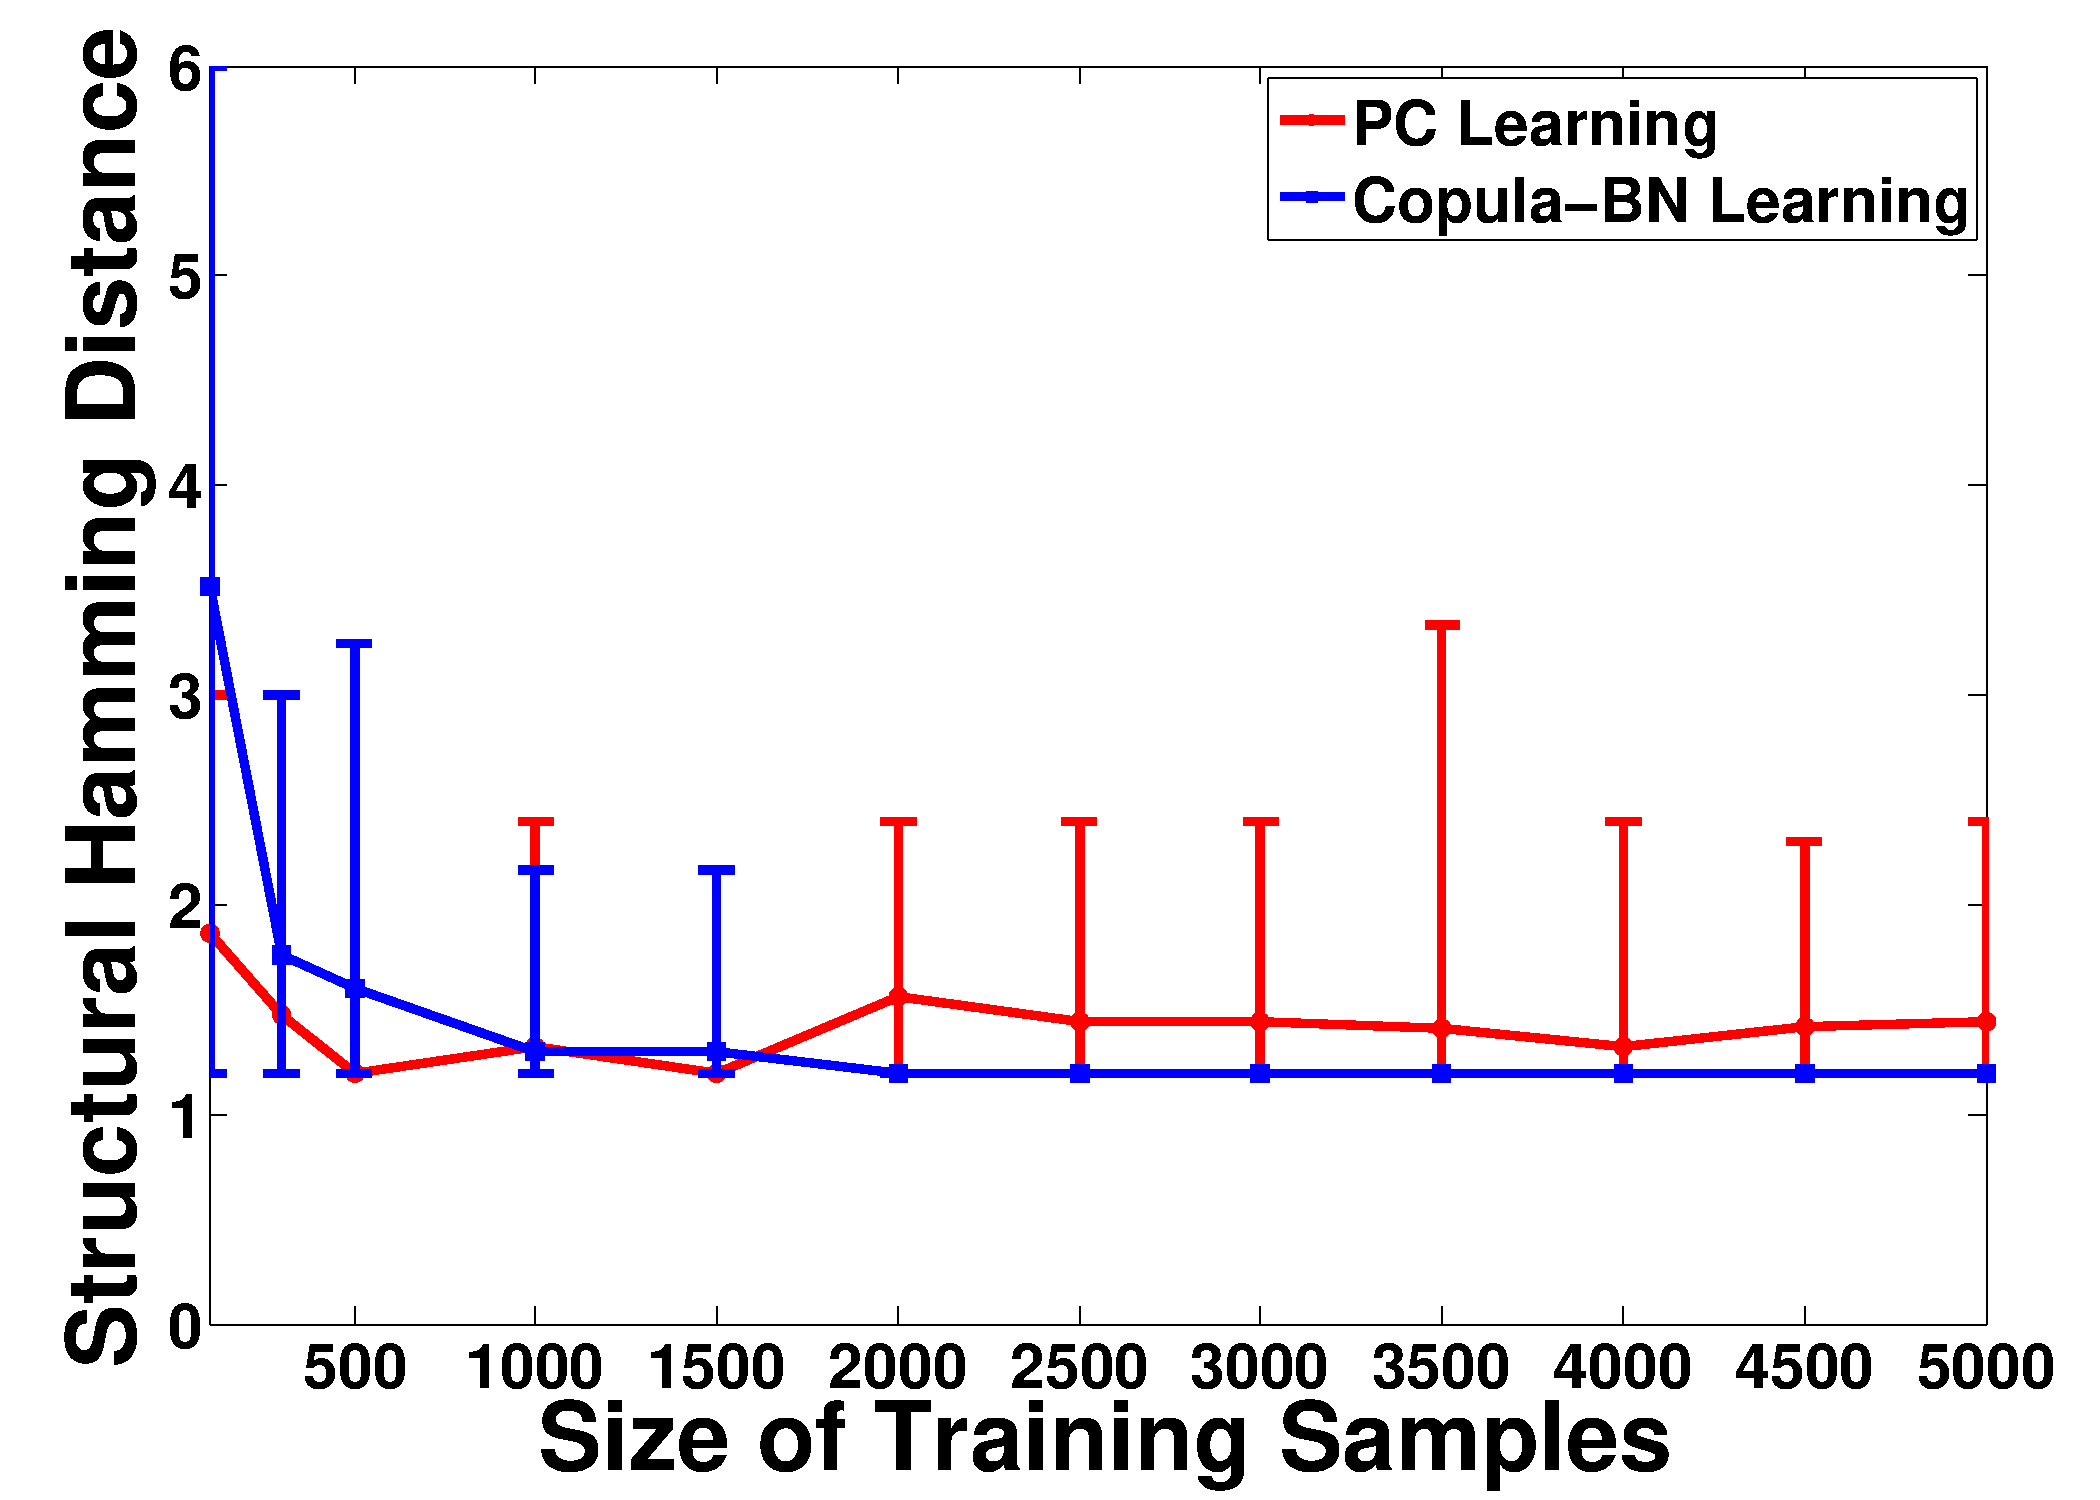
\includegraphics[width=0.24\textwidth]{Figures/plotsall/pc-copula-err5}}\\
\subfigure[7-nodes: runtime]{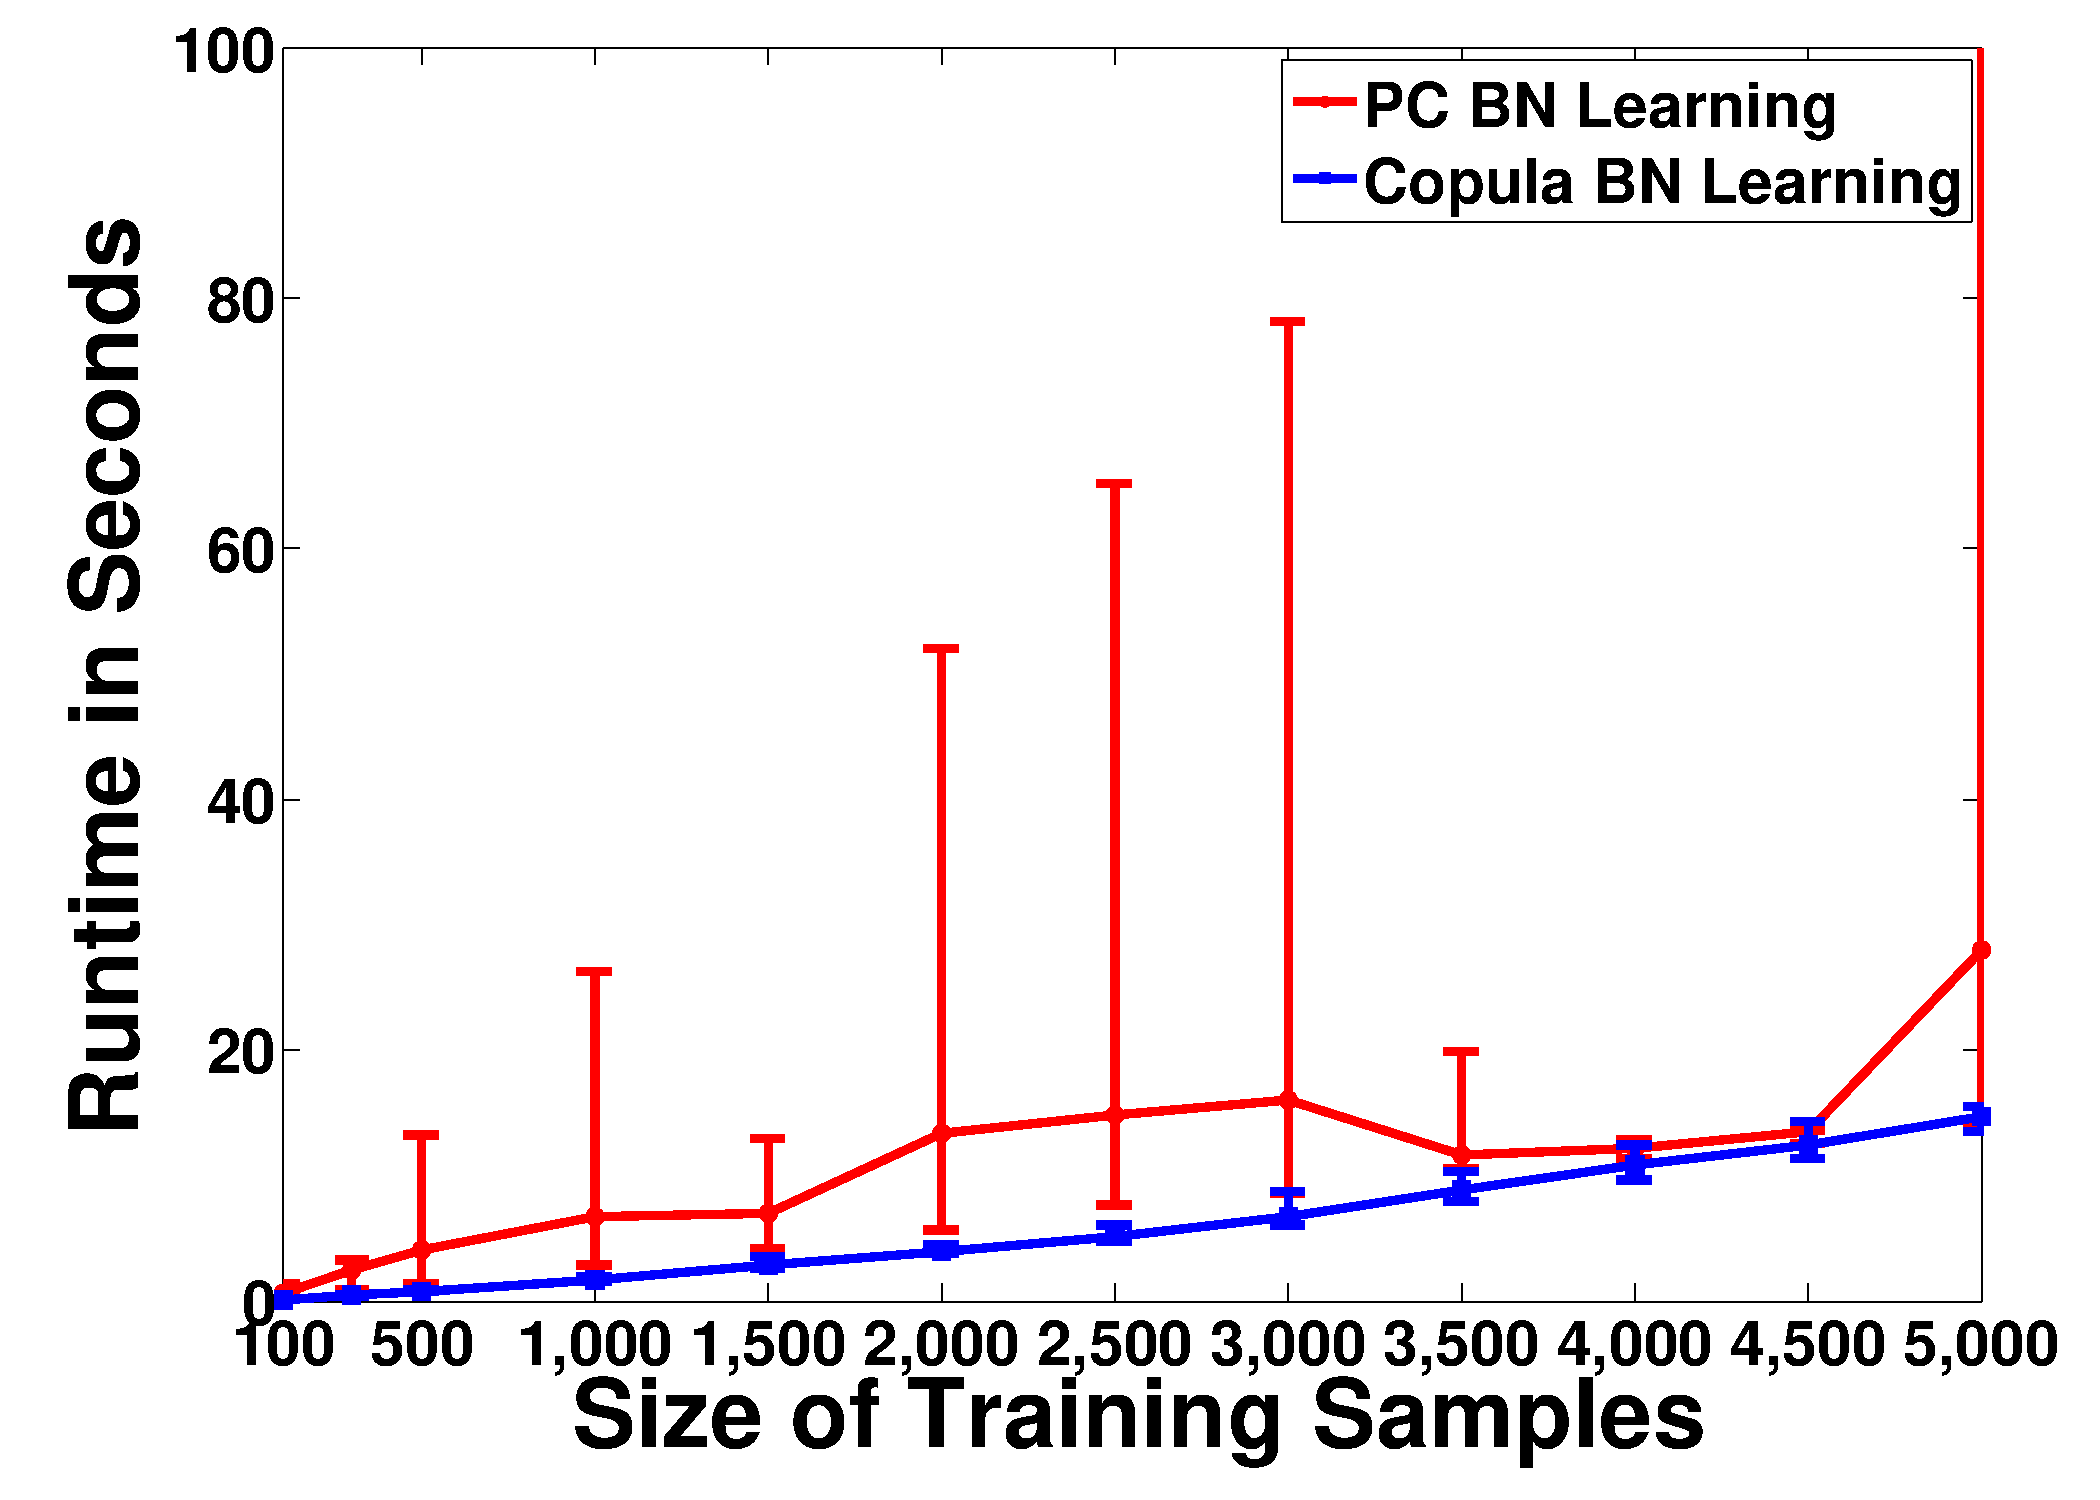
\includegraphics[width=0.24\textwidth]{Figures/plotsall/rtime-7err-f100}}\hfill
\subfigure[7-nodes: SHD error]{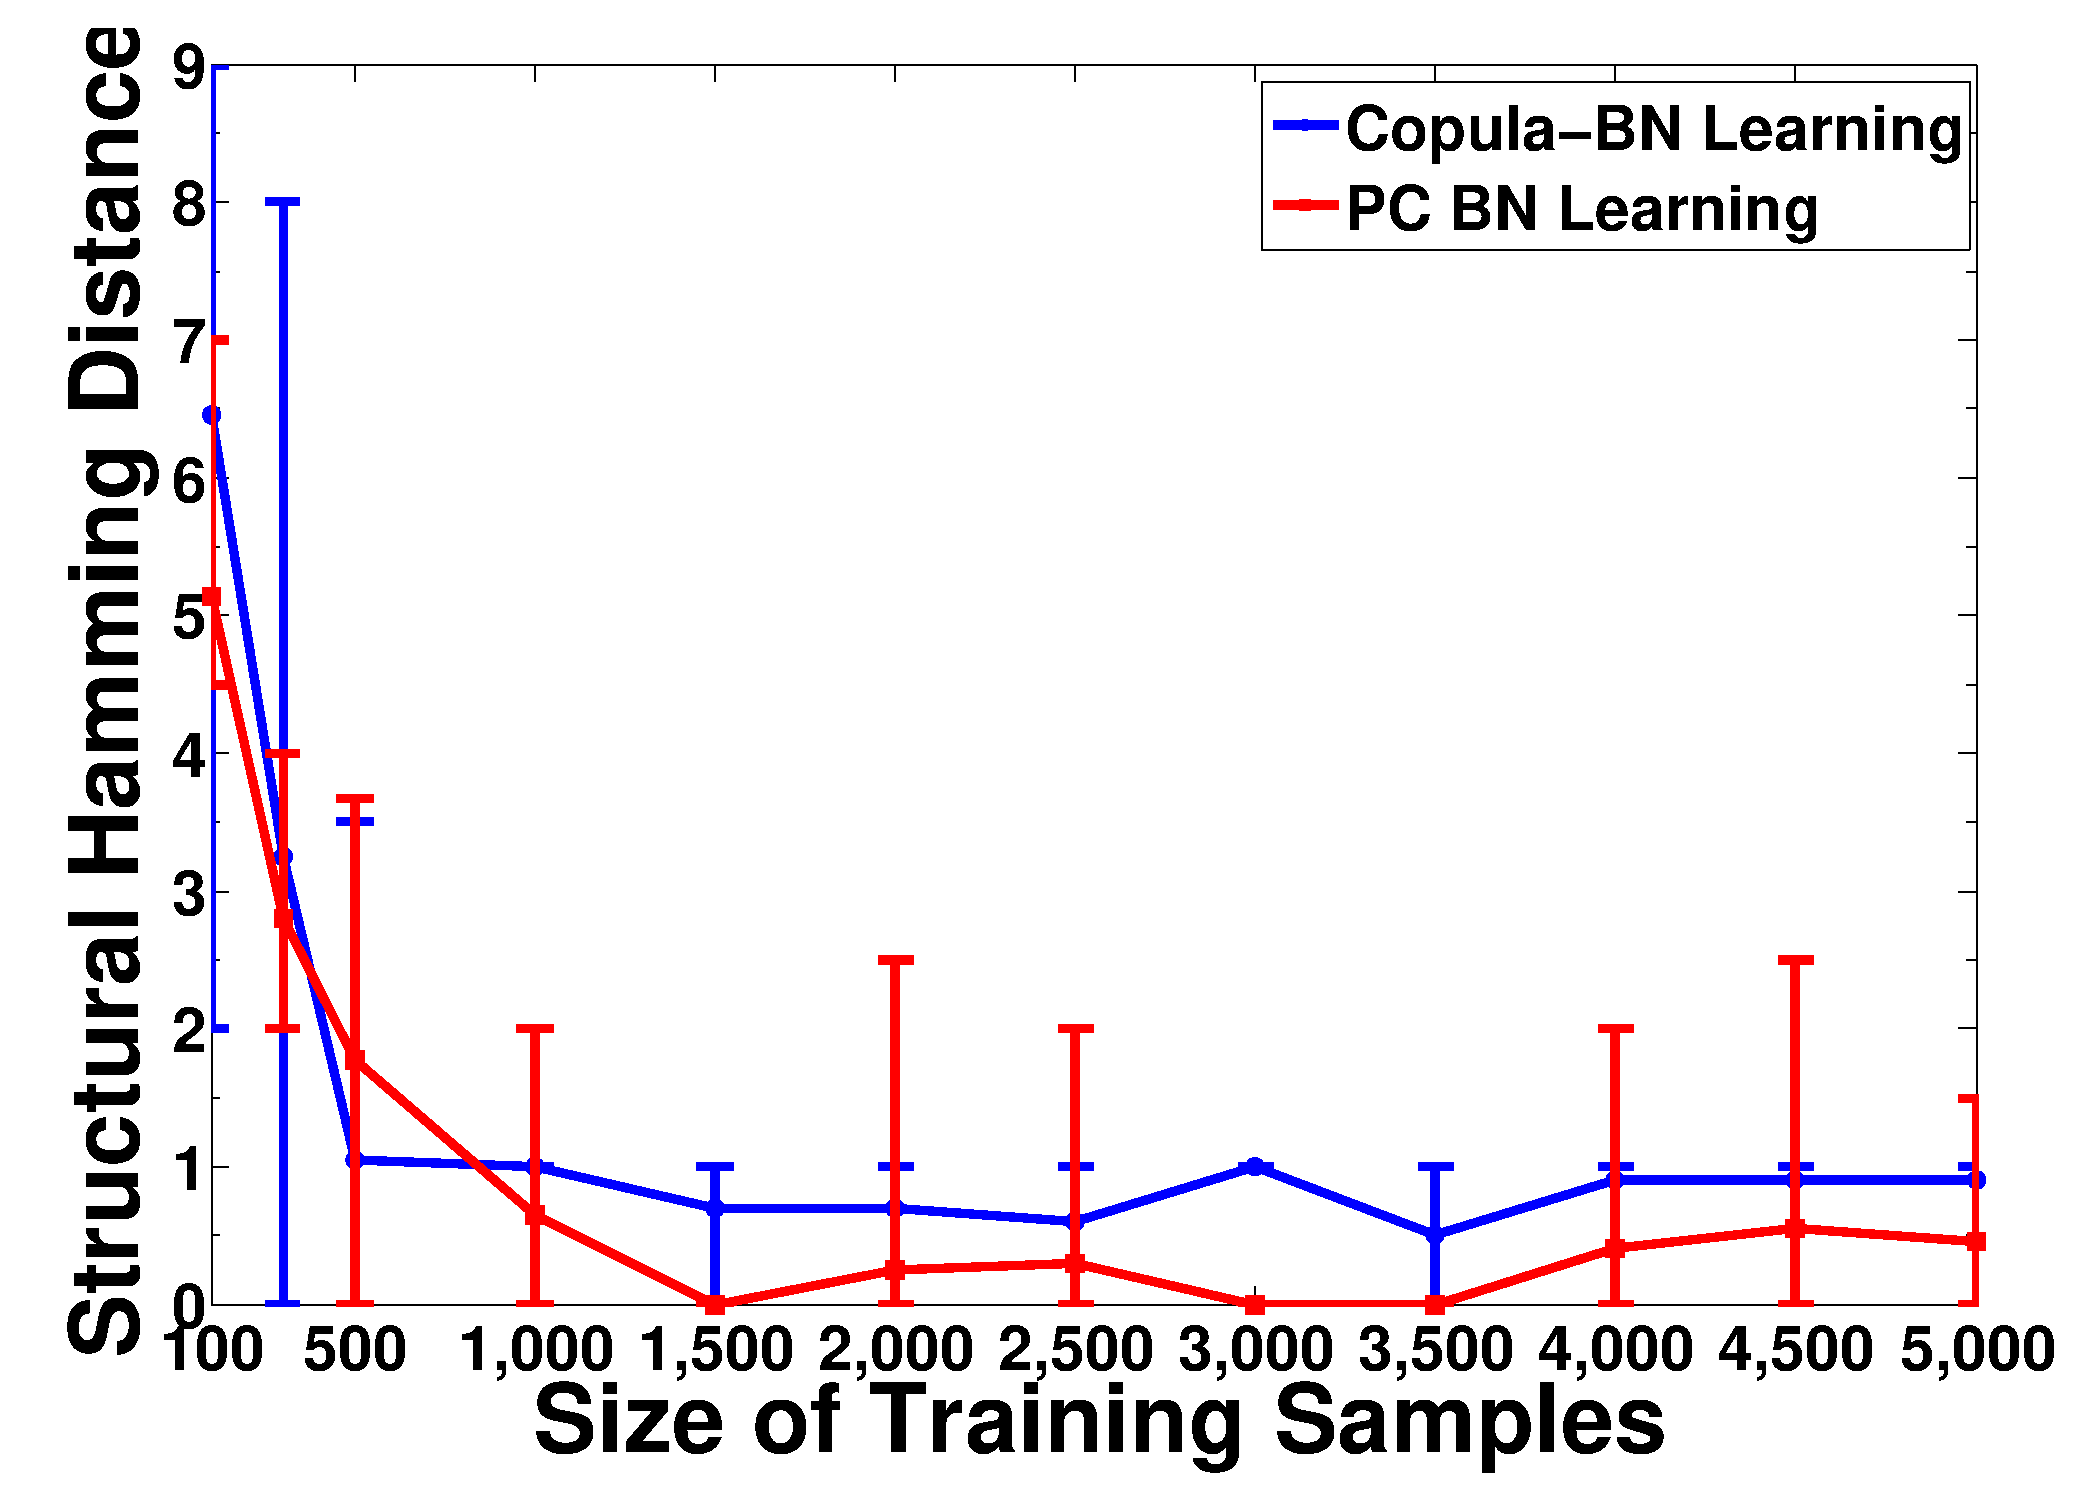
\includegraphics[width=0.24\textwidth]{Figures/plotsall/pc-copula-err7}}\\
\subfigure[10-nodes: runtime]{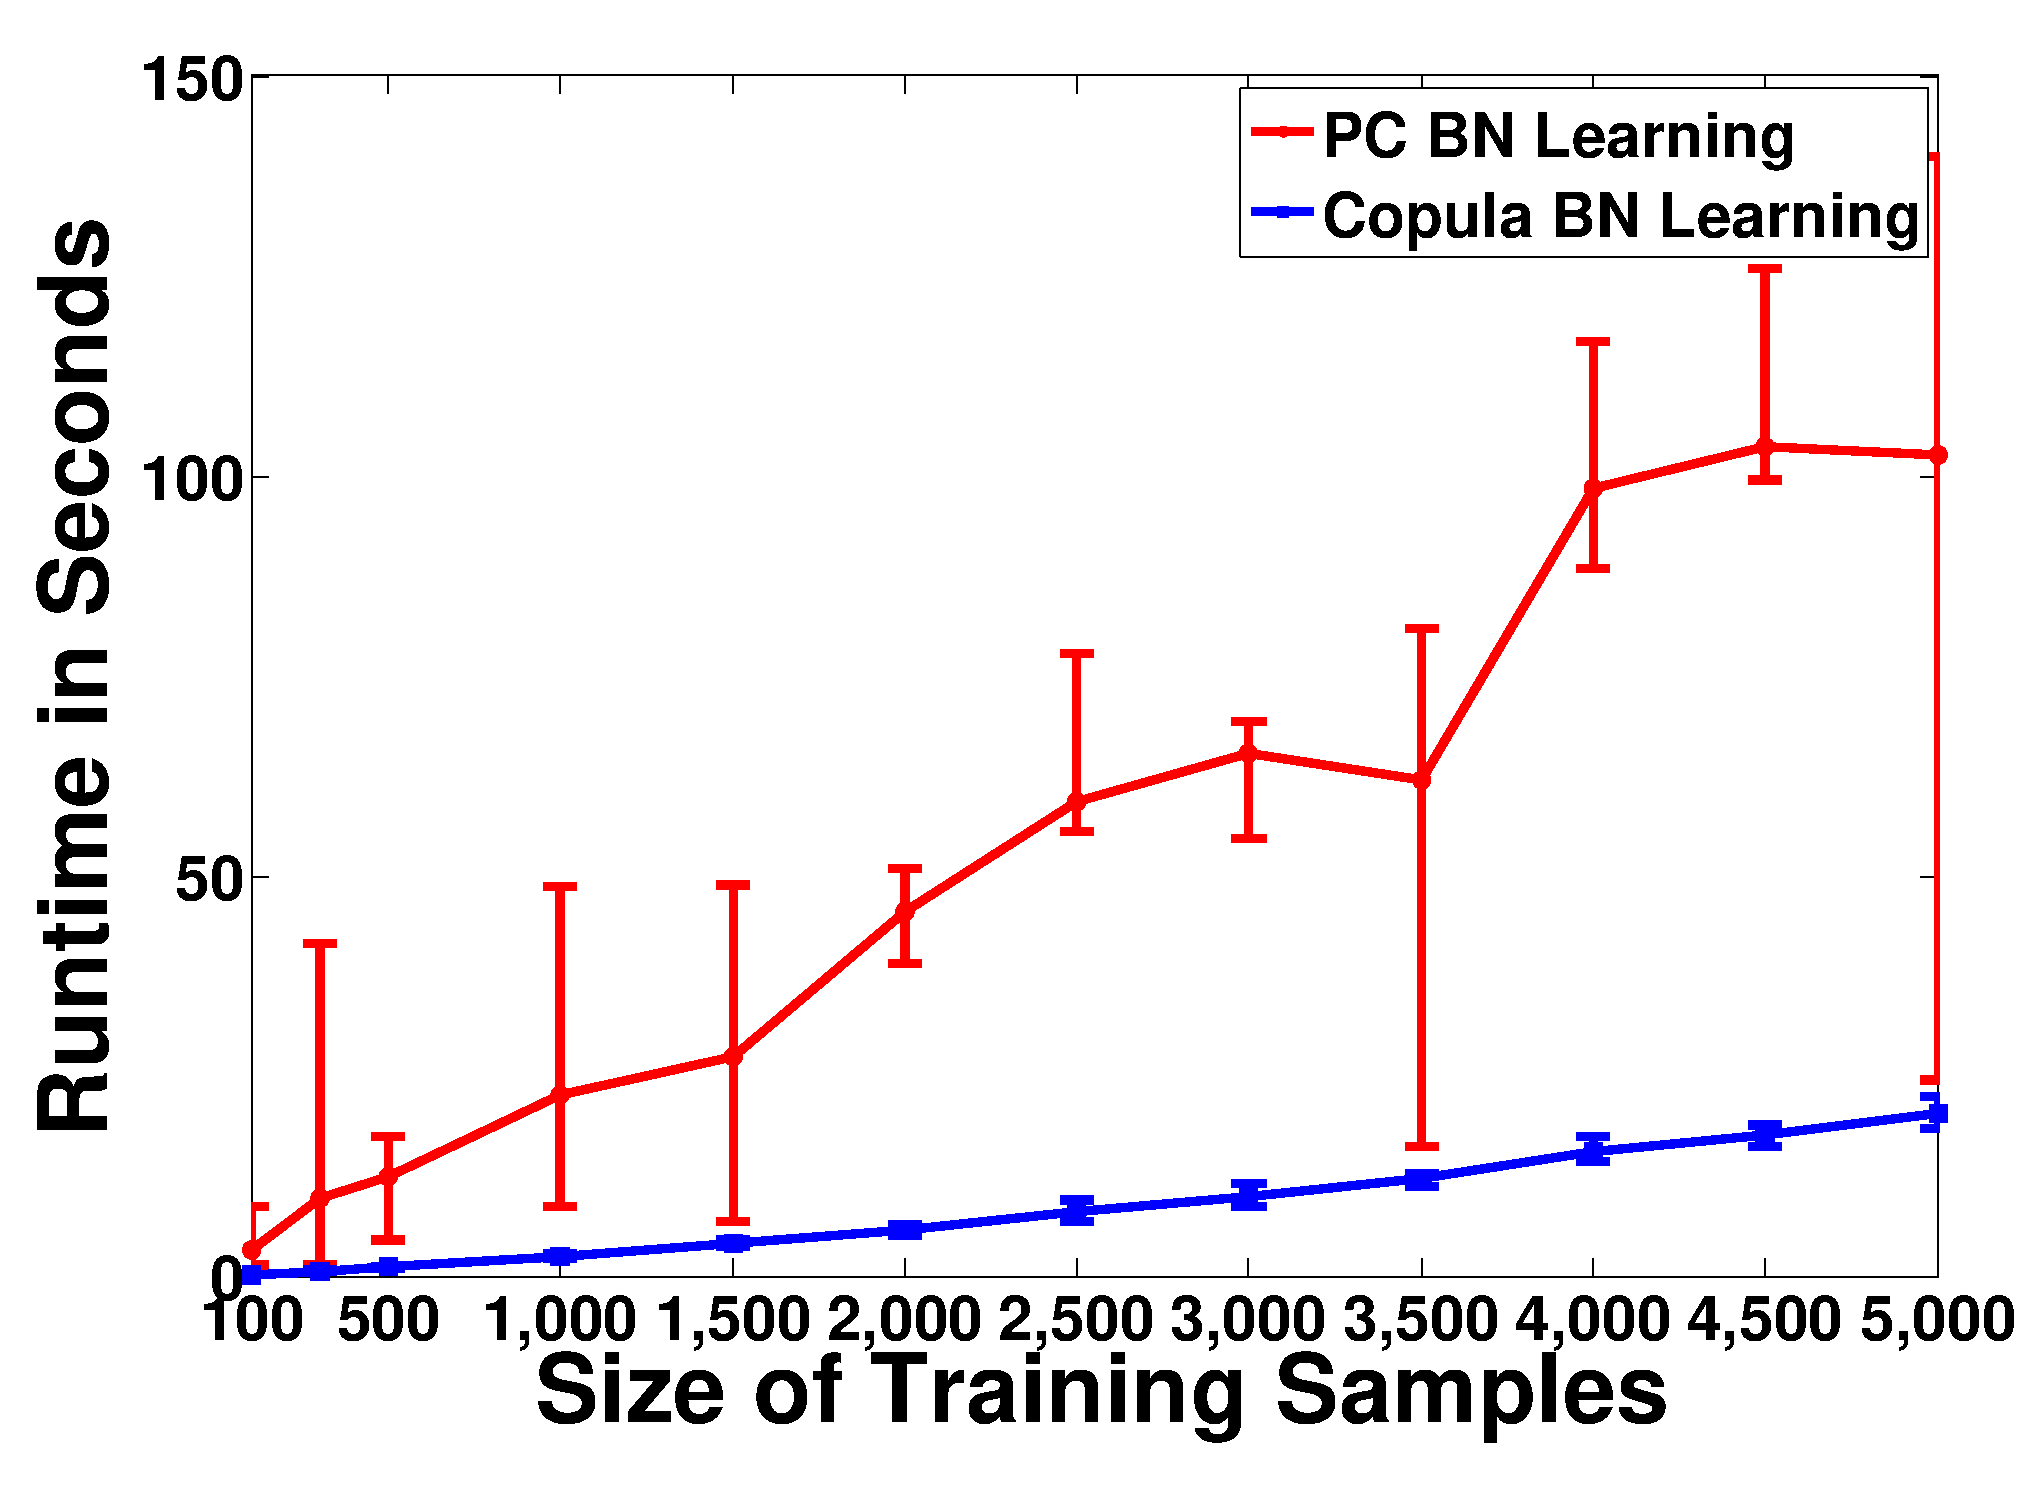
\includegraphics[width=0.24\textwidth]{Figures/plotsall/rtime-10err-f100}}\hfill
\subfigure[10-nodes: SHD error]{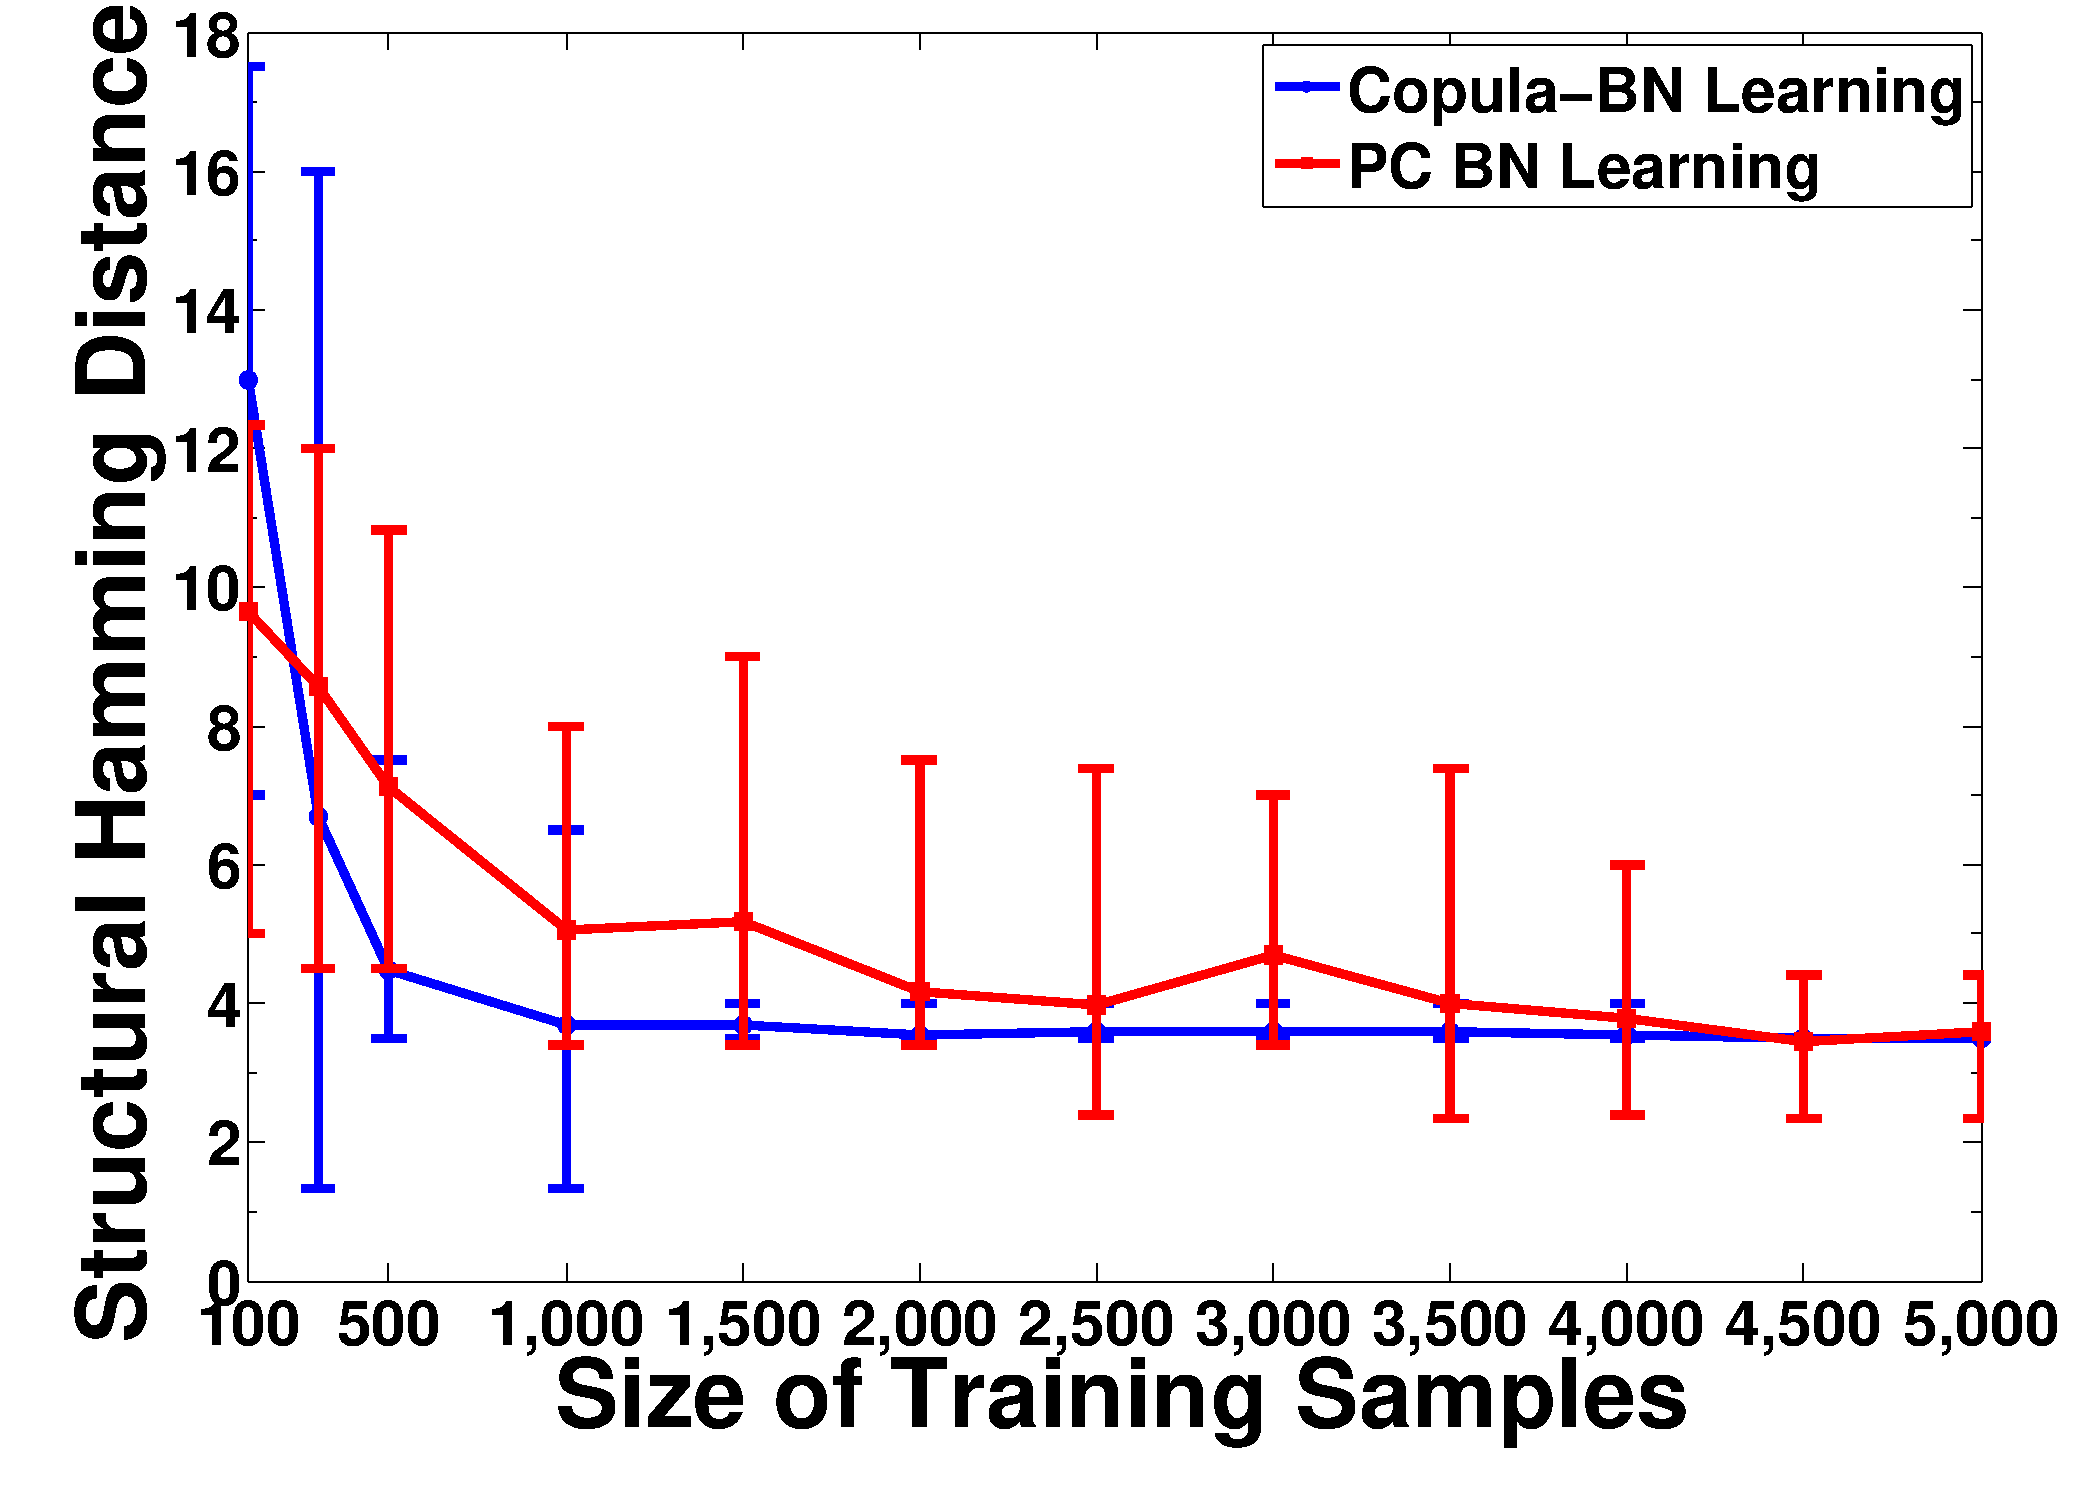
\includegraphics[width=0.24\textwidth]{Figures/plotsall/pc-copula-err10}}
\caption{Runtime and SHD error tests against various training sample sizes (range from 100 to 5000) on three synthetic networks (size 5,7,10), for PICM-CBN correlation thresholding $\sigma$ = 0.1, for the PC algorithm max-fan-in = 5 and PC thresholding $\alpha$ = 0.05.}
\label{fig:runtime}
\end{figure} 
%

% The original data set was used to predict the age of an abalone. 
This indicates that \textit{PICM-CBN} outperforms the PC algorithm regarding both the predictive accuracy and stability. Moreover, the results on the abalone data set looks quite attractive with roughly an average log-probability of $-1.7$ per instance for both training and test data sets.
\begin{figure}[H]
\centering
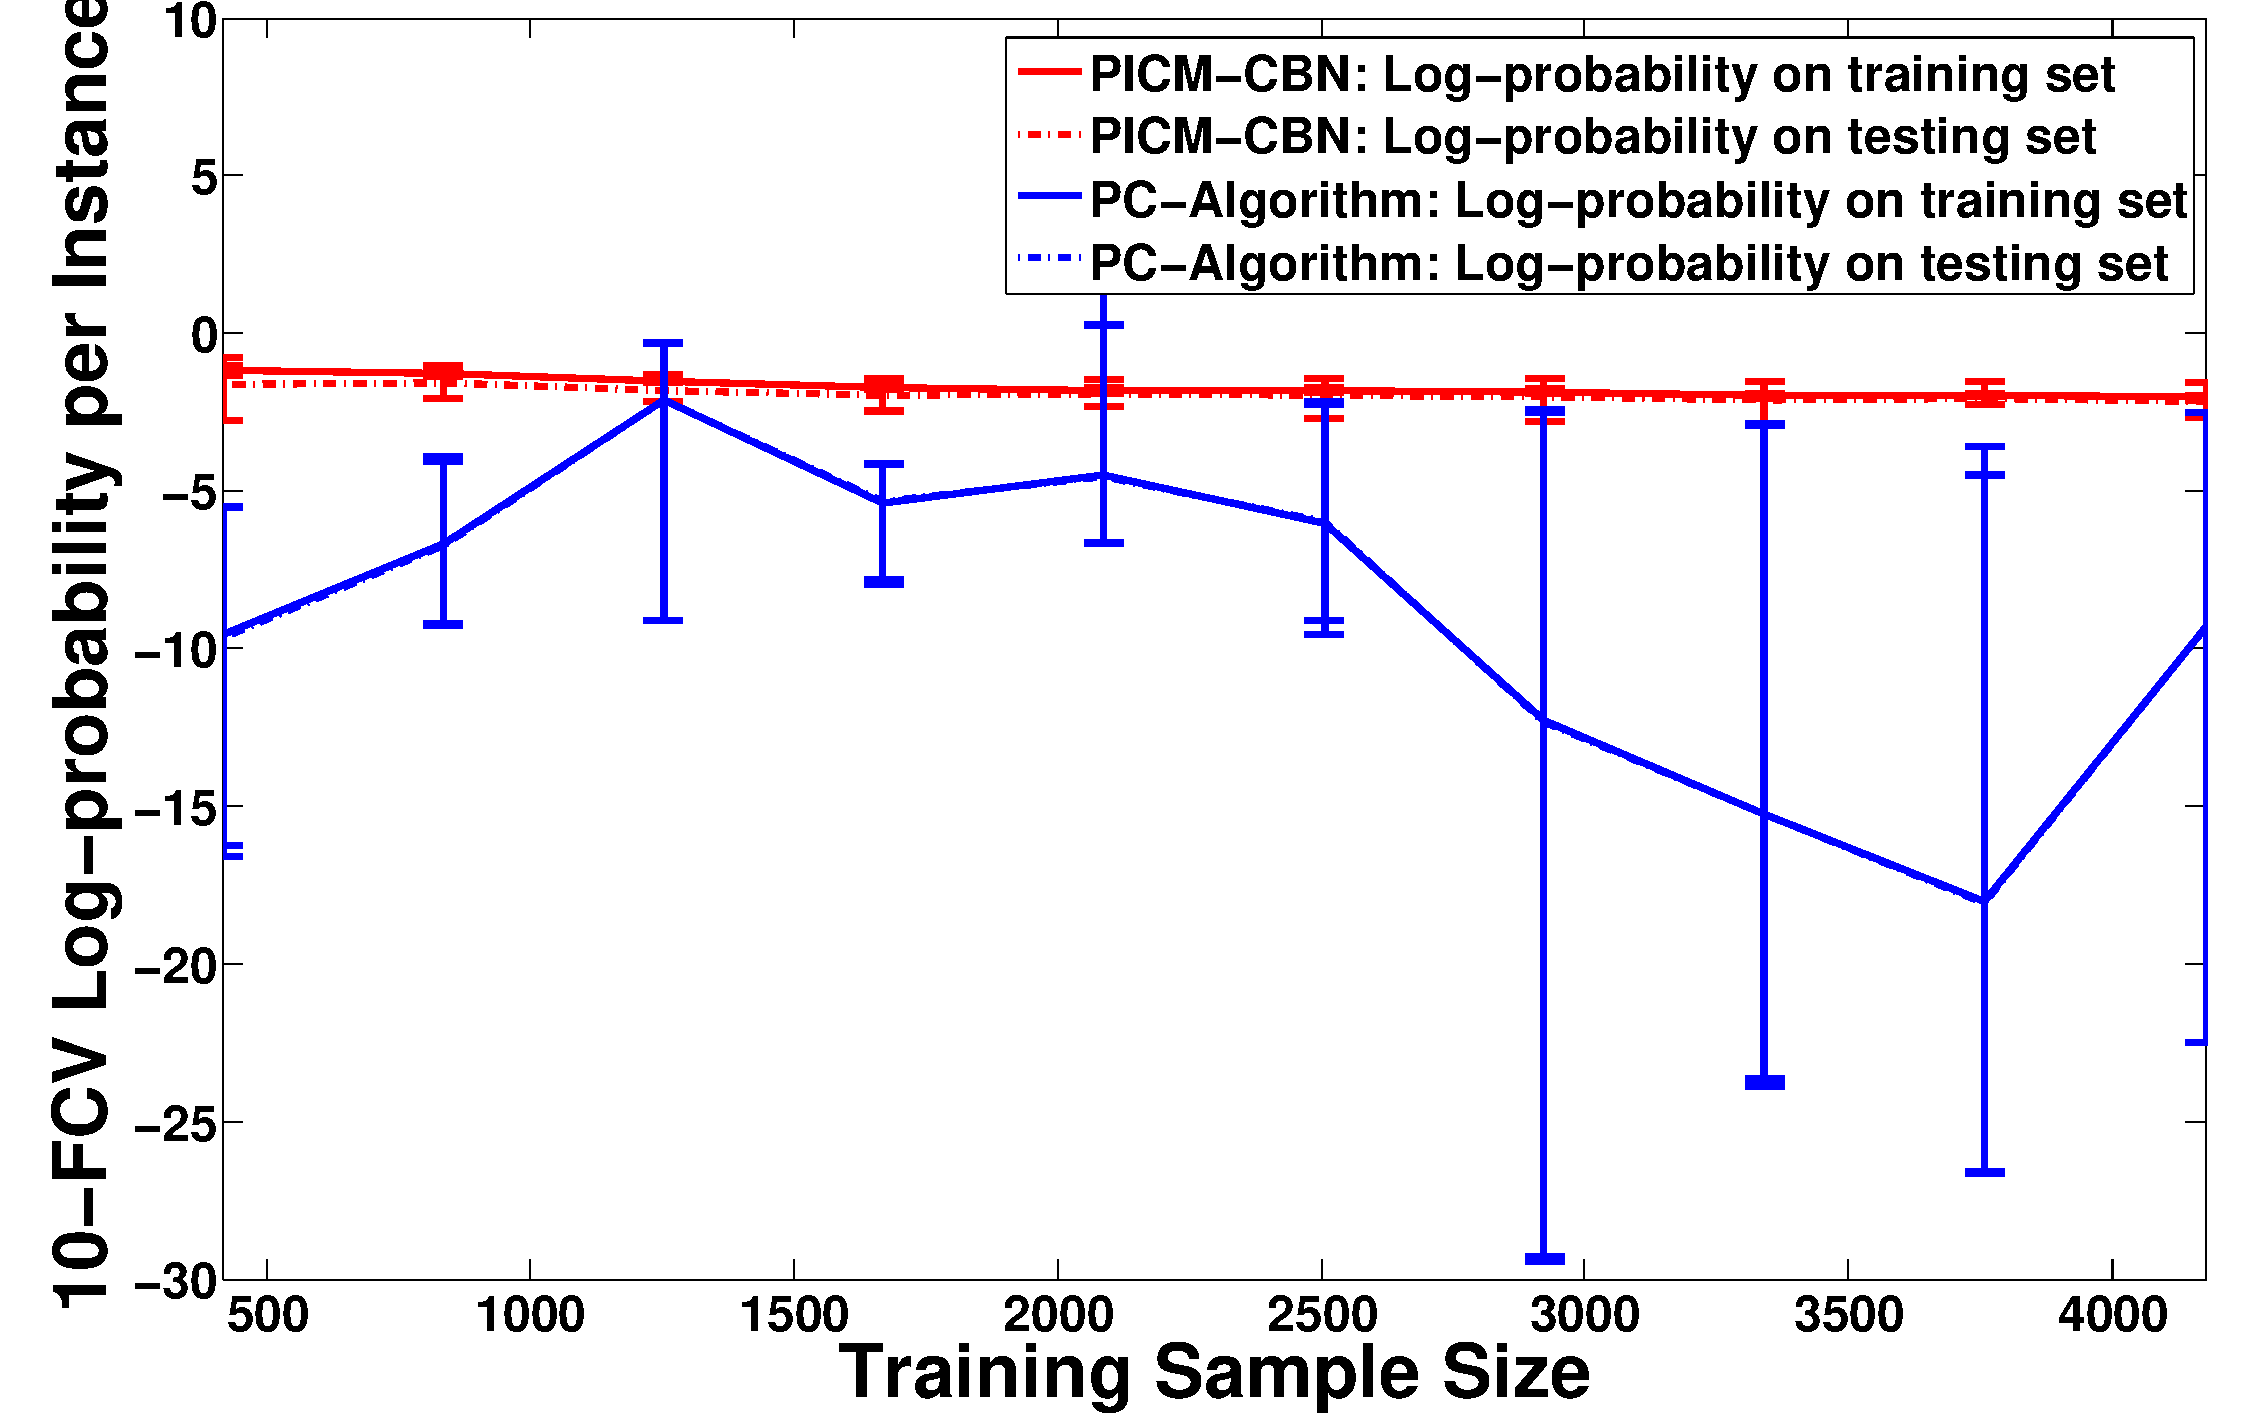
\includegraphics[width=0.4\textwidth]{Figures/plotsall/AbaloneSizeTrainTestLogPcCpl2}
\caption{Log-likelihood for the training and test set for \textit{PICM-CBN} and PC algorithms against 
	    the sample size on the Abalone data set (\textit{PICM-CBN}: $\sigma = 0.1$, PC: $\text{max-fan-in}=5, \alpha=0.05$).}
\label{fig:abalonelp}
\end{figure} 
In order to learn the network structure, we run \textit{PICM-CBN} multiple times on the full data set 
($\sigma=0.1$). The resulting % to construct a 
network structure with corresponding variable names is shown in %, as drawn in 
Figure \ref{fig:abaloneNetwork}. The learned network contains only 3 bidirectional edges and 12 edges 
in total. %It is apparent that t
\begin{figure} %[H]
\centering
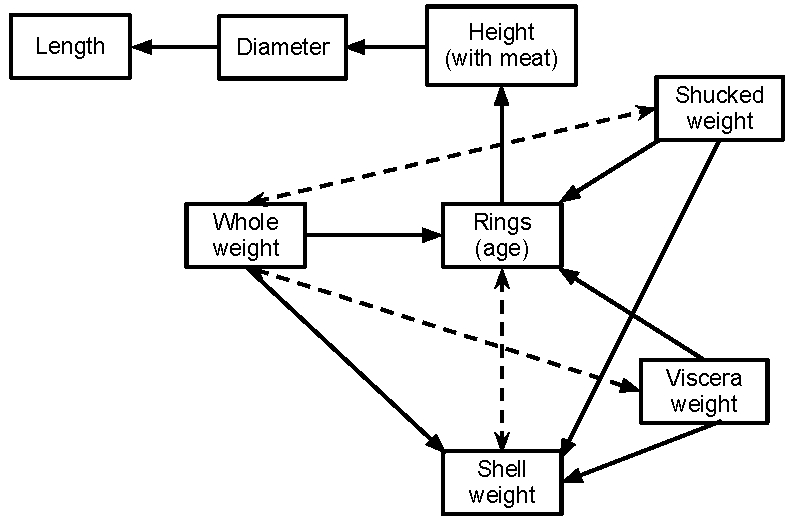
\includegraphics[width=0.35\textwidth]{Figures/AbaloneNetwork}
\caption{The learned network structure for Abalone data set.}
\label{fig:abaloneNetwork}
\vspace{-0.1in}
\end{figure}
The variable $\#rings$ located in the center possesses the most connections which 
implies that the age of abalone is impacted by most of the other given variables. For example, $\#rings$ is directly
 influenced by the abalone's $weight$, $shucked~weight$ and $viscera~weight$. The features regarding abalone's
 weight are highly connected, whereas the features about abalone's size including length and diameter are influenced
 by $\#rings$ (i.e., age). It is hard to assess the correctness of this causal model, but it corresponds
quite well to  prior knowledge about abalone.
%  the matter of fact at least by simply applying prior knowledge about abalone. 
Therefore, this model can also be used to predict the age of abalone given the other variables.
%

\section{Conclusion}
\label{sec:conc}
In this paper, we presented a new method for the induction of Copula Bayesian Networks
to model multivariate continuous distributions. 
%One important contribution of this approach is
%to use the partial inverse correlation matrix to reduce the number of
%dependence calculations among variables. 
We show that in Gaussian Copulas, instead of a large amount of independence tests, the PICM based structure learning method makes use of the estimated parameters of the Copula function to reduce the computational complexity. Experiments on the synthetic data sets show that our algorithm offers improvements on both structure learning and parameter learning.  
%show how to set a reasonable value for $\alpha$ (the correlation zero-approximation threshold)  and also show that the quality of
%the induced network increases for larger datasets but usually offers good results
%for datasets over 500 instances.
Moreover, comparisons to a BIC score heuristic-approach and the well known PC algorithm
suggest that the PICM-CBN algorithm comes to better results in less time.
% show that this approach may induce aqu
Furthermore, we showed that the induced network on a real life data set also gives reasonable results.
%
%
In the future, we first want to explore the impact of different families of Copulas on parameter estimation and
structure learning. Second, we would like to investigate the use of PICM-CBN for the reconstruction of gene regulatory networks.
%Since the high dimensionality and small sample
%size of the datasets are important characteristics, the applicability of PICM-CBN in such a scenario is to be
%evaluated.






\bibliography{literature} % use this
\bibliographystyle{icml2012}

\end{document} 


% This document was modified from the file originally made available by
% Pat Langley and Andrea Danyluk for ICML-2K. This version was
% created by Lise Getoor and Tobias Scheffer, it was slightly modified  
% from the 2010 version by Thorsten Joachims & Johannes Fuernkranz, 
% slightly modified from the 2009 version by Kiri Wagstaff and 
% Sam Roweis's 2008 version, which is slightly modified from 
% Prasad Tadepalli's 2007 version which is a lightly 
% changed version of the previous year's version by Andrew Moore, 
% which was in turn edited from those of Kristian Kersting and 
% Codrina Lauth. Alex Smola contributed to the algorithmic style files.  


